\documentclass[12pt, a4paper]{report}
\special{papersize=210mm, 297mm}
\usepackage[romanian]{babel}
\usepackage[utf8x]{inputenc}
\usepackage[left=2.5cm, right=2.5cm, top=2.5cm]{geometry}
\renewcommand{\baselinestretch}{1.4}
\usepackage[toc,page]{appendix}

\usepackage{amsmath}
\usepackage{graphicx}
\usepackage{float}
\graphicspath{{images/} {diagrams/}}

\usepackage{fullpage}
\usepackage{hyperref}
\usepackage{url}
\usepackage{listings}
\usepackage{verbatim}
\usepackage{color}
\usepackage{listings}
\usepackage{booktabs}
\usepackage{xcolor}

\definecolor{codegreen}{rgb}{0,0.6,0}

\lstset{frame=tb,
	 language=java,
	showstringspaces=false,
	columns=flexible, basicstyle={\small\ttfamily},
	numbers=none, numberstyle=\tiny\color{gray},
	keywordstyle=\color{blue},
	commentstyle=\color{dkgreen},
	stringstyle=\color{codegreen},
	morecomment=[f][\color{green}][0]{/},
	breakatwhitespace=true,
	tabsize=3
}

\usepackage{multirow}
\usepackage{array}
\newcolumntype{L}[1]{> {\raggedright\let\newline\\\arraybackslash\hspace{0pt}}m{#1}}
\newcolumntype{C}[1]{>{\centering\let\newline\\\arraybackslash\hspace{0pt}}m{#1}}
\newcolumntype{R}[1]{>{\raggedleft\let\newline\\\arraybackslash\hspace{0pt}}m{#1}}


\pagenumbering{roman}

\begin{document}
\renewcommand{\abstractname}{Abstract}
%======================================================================

\begin{titlepage}

	\newcommand{\HRule}{\rule{\linewidth}{0.5mm}} % Defines a new command for the horizontal lines, change thickness here

	\center % Center everything on the page

	%----------------------------------------------------------------------------------------
	%	LOGO SECTION
	%----------------------------------------------------------------------------------------

	\vspace{-20pt}
	
\includegraphics[width=100pt]{FMI-03.png}\\[1.0cm] % Include a department/university logo - this will require the graphicx package

	\textsc{\LARGE Universitatea de Vest din Timi\c{s}oara}\\[0.5cm] % Name of your university/college
	\textsc{\Large Facultatea de Matematic\u{a} \c{s}i Informatic\u{a}}\\[0.5cm] % Major heading such as course name
	\textsc{\large Domeniul de Studii: \\Informatic\u{a} Aplicat\u{a}}\\[3cm] % Minor heading such as course title

	%----------------------------------------------------------------------------------------
	%	TITLE SECTION
	%----------------------------------------------------------------------------------------

	\textsc{\Huge Lucrare de Diserta\c tie}\\[5cm]

	%\HRule \\[0.5cm]
	%{\huge \bfseries Simplified Transport Layer Security}
	%\\[0.4cm]
	%{\huge \bf implementation}\\[3cm] % Title of your document
	%\HRule \\[1.5cm]

	%----------------------------------------------------------------------------------------
	%	AUTHOR SECTION
	%----------------------------------------------------------------------------------------

	\begin{minipage}{0.4\textwidth}
		\begin{flushleft} \large
			\textbf{COORDONATOR:}\\
			Conf. Dr. Cristina \textsc{M\^ indru\c t\u a } % Coordinator
		\end{flushleft}
	\end{minipage}
	~
	\begin{minipage}{0.4\textwidth}
		\begin{flushright} \large
			\textbf{ABSOLVENT:} \\
			Nicolae \textsc{Savilencu} % Student's Name
		\end{flushright}
	\end{minipage}\\[1cm]


	%----------------------------------------------------------------------------------------
	%	DATE SECTION
	%----------------------------------------------------------------------------------------
	\vfill
	{\large Timi\c{s}oara \\2023}\\ % Date, change the \today to a set date if you want to be precise


	%----------------------------------------------------------------------------------------

	%\vfill % Fill the rest of the page with whitespace

\end{titlepage}

% =====================================================================

% second title page. as requested by UVT

\begin{titlepage}

	\newcommand{\HRule}{\rule{\linewidth}{0.5mm}} % Defines a new command for the horizontal lines, change thickness here

	\center % Center everything on the page

	%----------------------------------------------------------------------------------------
	%	LOGO SECTION
	%----------------------------------------------------------------------------------------

	%\vspace{-20pt}
	%
\includegraphics[width=100pt]{FMI-03.png}\\[1.0cm] % Include a department/university logo - this will require the graphicx package

	\textsc{\LARGE Universitatea de Vest din Timi\c soara}\\[0.5cm] % Name of your university/college
	\textsc{\Large Facultatea de Matematic\u a \c si Informatic\u a}\\[0.5cm] % Major heading such as course name
	% \textsc{\large Domeniul de Studii: \\Informatic\u a Aplicat\u a}\\[6cm] % Minor heading such as course title

	%----------------------------------------------------------------------------------------
	%	TITLE SECTION
	%----------------------------------------------------------------------------------------

	%\textsc{\Huge Master Dissertation}\\[2cm]

	\HRule \\[0.5cm]
	{\Huge \bf Tehnologii de randare a informa\c tiilor \^ in aplica\c tiile web moderne}\\[6cm] % Title of your document
	%\HRule \\[1.5cm]

	%----------------------------------------------------------------------------------------
	%	AUTHOR SECTION
	%----------------------------------------------------------------------------------------

	%\textsc{\huge Intermediate Report}

	\begin{minipage}{0.4\textwidth}
		\begin{flushleft} \large
			\textbf{COORDONATOR:}\\
			Conf. Dr. Cristina \textsc{M\^ indru\c t\u a} % Coordinator
		\end{flushleft}
	\end{minipage}
	~
	\begin{minipage}{0.4\textwidth}
		\begin{flushright} \large
			\textbf{ABSOLVENT:} \\
			Nicolae \textsc{Savilencu} % Student's Name
		\end{flushright}
	\end{minipage}\\[1cm]

	%----------------------------------------------------------------------------------------
	%	DATE SECTION
	%----------------------------------------------------------------------------------------
	\vfill
	{\large Timi\c soara\\ 2023}\\ % Date, change the \today to a set date if you want to be precise


	%----------------------------------------------------------------------------------------

	%\vfill % Fill the rest of the page with whitespace

\end{titlepage}

\begin{abstract}
	%The abstract should have one page and should be a compact presentation of the dissertation.
	\vspace{1.0cm}
	\par
	The web is evolving at a rapid pace, and with the emergence of new web technologies, the way web applications are built has changed significantly compared to the structures used in the past. Rendering is a critical aspect of web development, and modern web applications require faster, more efficient rendering techniques to deliver a better user experience. This dissertation aims to explore the rendering technologies used in modern web applications in order to define an optimal yet flexible solution for developing applications of different scales.

	The research begins by introducing the fundamental concepts of web rendering, including two of the most known approaches: server-side rendering and client-side rendering. It then examines the evolution of rendering technologies, from traditional rendering techniques with HTML, CSS, and JavaScript, to modern technologies like React, Gatsby, and Next. The dissertation compares and contrasts these technologies and analyzes their performance and usability by some predefined metrics: LCP (\emph{Largest Contentful Paint}), FID (\emph{First Input Delay}), CLS (\emph{Cumulative Layout Shift}), and other important factors such as development time and scaling ability.
	
	The dissertation explores the impact of rendering technologies on development workflows and examines the challenges associated with adopting new technologies, such as the learning curve, compatibility issues, performance bottlenecks, and SEO optimization.
	
	Finally, the dissertation provides a case study of a web application built using multiple technologies, comparing the performance metrics of each individual technology's advantages and disadvantages.
	
	Overall, the dissertation provides a comprehensive analysis of rendering technologies in modern web applications and their impact on web development to identify the most optimal methods of creating performant, scalable, and user-friendly applications.

\end{abstract}

\tableofcontents{}
\addcontentsline{toc}{chapter}{List\u a de figuri}
\listoffigures{}

\newpage{}

\chapter{Introducere}

\pagenumbering{arabic}
\setcounter{page}{1}


\section{Motiva\c tie \c si scop}

Obiectivul acestei lucr\u ari este de a analiza tehnologiile de randare utilizate \^in aplica\c tiile web moderne, pentru a identifica metode de dezvoltare optime, din punct de vedere al performan\c tei, experien\c tei utilizatorului \c si SEO (Search Engine Optimization). Aceste rezultate vor fi ob\c tinute prin compararea mai multor framework-uri front-end dup\u a un anumit set de criterii, prestabilit, prin intermediu dezvolt\u arii unei aplica\c tii, cu fiecare dintre aceste framework-uri, pentru a identifica cele mai eficiente \c sabloane de dezvoltare.

Motiva\c tia alegerii acestei teme de diserta\c tie deriv\u a din mai mul\c ti factori. \^In primul r\^and, progresul tehnologic rapid a dus la apari\c tia mai multor paradigme de dezvoltare a aplica\c tiilor web, iar \c tinerea pasului cu acestea a devenit o provocare. \^In al doilea r\^and, odat\u a cu crearea unor aplica\c tii din ce \^in ce mai complexe, necesitatea de a cunoa\c ste procesele interne precum tehnologiile \c si metodele de randare a devenit o component\u a esen\c tial\u a a dezvolt\u arii. Prin urmare, \^in\c telegerea modului \^in care func\c tioneaz\u a aceste tehnologii \c si a modului \^in care acestea pot fi optimizate poate ajuta la dezvoltarea unei aplica\c tii care ar oferi o experien\c t\u a de utilizare \c si o performan\c t\u a sporit\u a.

\^In cele din urm\u a, aceast\u a lucrare de diserta\c tie \^i\c si propune s\u a ofere informa\c tii despe tehnologiile de randare utilizate \^in aplica\c tiile web moderne \c si despre impactul acestora asupra performan\c tei, pentru a identifica cele mai eficiente framework-uri pentru a dezvolta o aplica\c tie web ce poate fi scalat\u a, bine optimizat\u a \c si cu un UX (User Experience) de nivel \^inalt.


\section{Contextul lucr\u arii}


World Wide Web nu este un sinonim al internetului, dar este cea mai proeminent\u a parte a acestuia, care poate fi definit\u a ca un sistem tehno-social cu care interac\c tioneaz\u a oamenii prin intermediul re\c telelor tehnologice. No\c tiunea de sistem tehno-social se refer\u a la un sistem care \^imbun\u at\u a\c te\c ste percep\c tia uman\u a, comunicarea \c si cooperarea. Percep\c tia este condi\c tia prealabil\u a necesar\u a pentru a comunica \c si coopera.

Pe 12 Martie 1989, Tim Berners-Lee, informatician de origine britanic\u a \c si un fost angajat CERN au scris o propunere pentru ceea ce va deveni ulterior World Wide Web. Acea propunere avea drept scop crearea unui sistem de comunica\c tii mai eficient \^in cadrul CERN, \^ins\u a Berners-Lee a realizat \^in cele din urm\u a c\u a conceptul ar putea fi implementat la scar\u a global\u a. \^Impreun\u a cu informaticianul belgian Robert Cailliau au propus \^in 1990 s\u a folosesac\u a hypertext pentru a lega \c si accesa diverse tipuri de informa\c tii dintr-o re\c tea de noduri \^in care utilizatorul poate naviga c\u atre rezultatele dorite.

Prima versiune a web-ului global de la CERN a fost construit\u a pe primele versiuni ale HTTP (HyperText Transfer Protocol) \c si HTML (HyperText Markup Language). Aceste pagini web au fost servite de primul server web. Berners-Lee a scris, de asemenea, primul browser web pentru a accesa acest nou web creat. Web-ul global s-a schimbat drastic de la concep\c tia sa original\u a din 1989.

\subsection{Web 1.0}

A fost creat \^in 1989 \c si utilizat p\^an\u a \^in 2005. Potrivit lui Tim Berners-Lee Web 1.0 a fost \emph{read-only}, deoarece oferea foarte pu\c tin\u a interac\c tiune pentru utilizatori. Rolul web-ului a fost de natur\u a pasaiv\u a.

Web 1.0 a fost prima genera\c tie de World Wide Web \c si con\c tinea doar pagini statice ce aveau doar un singur scop - de livrare a con\c tinutului. Deoarece era monodirectional, \^ insemna c\u a organiza\c tiile \^ imp\u art\u a\c seau informa\c tii precum bro\c suri, cataloage \^ doar pentru citire. Aceste date erau prezentate pe pagini HTML statice care se modificau manual. Utilizatorii nu puteau contribui la paginile web existente. Tehnologiile Web 1.0 includ protocoale web de baz\u a, HTML, HTTP \c si URI. \cite{web-1}

Browserele erau foarte rudimentare \c si site-urile web erau mici. De aceea era destul s\u a se creeze un fi\c sier HTML static care ar con\c tine toate datele necesare \c si designul, care nu ar fi fost niciodat\u a actualizate automat.
\begin{lstlisting}[caption={Exemplu fi\c sier HTML},captionpos=b]
	!DOCTYPE html>
	<html>
		<head>
			<title>Page Title</title>
		</head>
		<body>
			<h1>Heading example</h1>
			<p>My first paragraph.</p>
		</body>
	</html>
	
\end{lstlisting}

Mai t\^ arziu, c\^ and browser-ele au dezvoltat capacit\u a\c ti vizuale, a aparut necesitatea de stilizare. Håkon W Lie a propus o prima versiune a CSS (Cascading Style Sheet), care este folosit \c si \^ in prezent. Acesta este un limbaj de stilizare folosit pentru a descrie modul \^ in care un document HTML ar trebui s\u a fie prezentat. CSS a fost creat pentru a permite separarea con\c tinutului \c si a prezent\u arii. Acest lucru a permis paginilor web s\u a fie mai accesibile, mai u\c sor de \^intre\c tinut \c si mai flexibile.
\begin{lstlisting}[caption={Exemplu fi\c sier CSS},captionpos=b]
	body {
		background-color: black;
		margin: 10px 5px;
	}

	p {
		font-size: 12px;
		color: red;
	}
\end{lstlisting}

\textbf{Caracteristici:}
\begin{itemize}
	\item Con\c tinut read-only
	\item Informa\c tiile erau la dispozi\c tia oricui \c si oric\^and
	\item Include pagini web statice \c si utilizeaz\u a HTML
\end{itemize}

\textbf{Limit\u ari:}
\begin{itemize}
	\item Paginile puteau fi \^in\c telese doar de oameni \c si nu aveau con\c tinut compatibil pentru motoare de c\u autare
	\item Utilizatorii erau responsabili pentru responsabili pentru actualizarea \c si gestionarea con\c tinutului
	\item Incapabilitatea de a reprezenta informa\c tii dinamice
\end{itemize}

\subsection{Web 2.0}

Tim O'Reilly a definit Web 2.0 drept fiind revolu\c tia afacerilor \^ in industria calculatorului, cauzat\u a de mutarea c\u atre internet ca platform\u a \c si \^ incercarea de a \^ in\c telege regulile pentru succes pe aceast\u a nou\u a platform\u a. Printre aceste reguli se num\u ar\u a urm\u atoarea: construirea de aplica\c tii care s\u a valorifice efectele de re\c tea pentru a deveni mai bune pe m\u asur\u a ce mai mul\c ti oameni le folosesc. \cite{oreilly}

Web 2.0 faciliteaz\u a propriet\u a\c ti majore cum ar fi practicile participative, colaborative \c si distribuite, care permit desf\u a\c surarea activit\u a\c tilor zilnice formale \c si \^in sfere formale pe web. Web 2.0 este web-as-a-platform. Utilizatorii au mai multe unelte pentru interac\c tiune, \^ins\u a cu mai pu\c tin control. Versiunea 2.0 implic\u a \c si un design web flexibil, reutilizare creativ\u a, actualiz\u ari \c si creare de con\c tinut colaborativ, care este considerat\u a una dintre cele mai remarcabile caracteristici ale web 2.0.

\^ Impreun\u a cu primele site-uri web dinamice a venit nevoia pentru primele tehnologii de programare pe partea de server. La \^ inceput, programarea pe partea de server se f\u acea direct \^ in serverul web. Mai t\^ arziu, standardul CGI (Common Gateway Interface) a fost dezvoltat, ceea ce a f\u acut posibil\u a interac\c tiunea serverului web cu orice proces local.
Mai t\^ arziu, limbi precum Perl, Java, PHP \c si ASP (\c si altele) au devenit populare pentru programare pe partea de server.

Site-urile web care devin mai bogate \^ in func\c tii au nevoie de mai mult\u a flexibilitate \c si de o utilizare mai bun\u a. Acesta este momentul \^ in care programarea client-side intr\u a \^ in joc. F\u ar\u a a fi nevoie de o \^ inc\u arcare complet\u a a paginii, con\c tinutul poate fi schimbat de c\u atre utilizatorii finali. Tehnologia cel mai utilizat\u a pentru acest scop este JavaScript.
C\^ and func\c tiile client-side au devenit \c si mai importante, au fost concepute framework-uri pentru randarea (\c si controlarea) paginilor client-side. Cele mai cunoscute framework-uri sunt: Ember, Angular \c si React.

\textbf{Caracteristici:}
\begin{itemize}
	\item Web-ul a devenit o platform\u a cu software peste nivelul unui singur dispozitiv
	\item Trecerea la internet-as-a-platform \c si \^incercarea de a \^in\c telege regulile succesului \^in aceast\u a nou\u a platform\u a
	\item Social Web este adesea folosit pentru a caracteriza site-urile care constau din comunit\u a\c ti. Este bazat pe content management \c si identificarea unor noi metode de comunicare \c si interac\c tionare dintre utilizatori. Aplica\c tia web faciliteaz\u a producerea colectiv\u a de cuno\c stin\c te, re\c tele sociale \c si cre\c ste rata de schimb de informa\c tii dintre utilizatori
\end{itemize}


\textbf{Limit\u ari:}
\begin{itemize}
	\item Ciclu constant de itera\c tii a schimbarilor \c si actualiz\u arilor serviciilor
	\item Probleme etice privind construirea \c si utilizarea web 2.0
	\item Interconectivitatea \c si schimbul de cuno\c stin\c te \^intre platforme dincolo de grani\c tele comunit\u a\c tii sunt \^inc\u a limitate
\end{itemize}

\subsection{Web 3.0}

Cunoscut \c si sub numele de web semantic sau Web decentralizat, este urm\u atoarea genera\c tie a World Wide Web, care \^i\c si propune s\u a ofere o experien\c t\u a mai inteligent\u a, interconectat\u a \c si decentralizat\u a. Reprezint\u a o viziune pentru viitorul web \^in care datele, aplica\c tiile \c si serviciile sunt interconectate \^in mod fluid, permi\c t\^and ma\c sinilor \c si oamenilor s\u a \^in\c teleag\u a \c si s\u a interac\c tioneze mai eficient cu informa\c tiile.

Ideea ce se afl\u a la baz\u a este de a defini structurile de date \c si de a le lega pentru o automatizare, intregare \c si reutilizare mai eficient\u a \^in diverse aplica\c tii. Web 3.0 este capabil s\u a \^imbun\u at\u a\c teasc\u a gestionarea datelor, s\u a sus\c tin\u a accesibilitatea internetului mobil, s\u a stimuleze creativitatea \c si inova\c tia, s\u a \^incurajeze fenomenul de globalizare, s\u a sporeasc\u a experien\c ta utilizatorilor \c si s\u a ajute la organizarea colabor\u arii \^in re\c telele sociale. \cite{semantic-web}

\^In 3.0 conceptul de site web \c si pagin\u a web dispare, datele nu sunt de\c tinute, ci partajate, iar serviciile afi\c seaz\u a diferite vederi, pe baza datelor. Aceste servicii pot fi aplica\c tii \c si trebuie s\u a se concentreze pe context \c si personalizare, ce vor fi atinse prin utilizarea c\u autarilor verticale. Web 3.0 faciliteaz\u a dezvoltarea de aplica\c tii care utilizeaz\u a inteligen\c ta artificial\u a, \^inv\u a\c tarea automat\u a \c si procesarea limbajului natural. Aceste tehnologii permit analiza avansat\u a a datelor, automatizarea \c si capacitatea de luare a deciziilor, rezult\^and \^in servicii mai inteligente \c si personalizate pentru utilizatori.

Urm\u atorul pas \^ in dezvoltarea web-ului este crearea aplica\c tiilor web autonome, care pot fi, de asemenea, utilizate f\u ar\u a conexiune la internet. Acestea sunt numite Aplica\c tii Web Progressive (PWA). Crearea acestor aplica\c tii nu este posibil\u a f\u ar\u a a avea control complet la nivelul clientului. Randarea pe partea de server nu este posibil\u a \c si se folosesc framework-uri complete pentru front-end pentru a construi acest fel de aplica\c tii. Comunicarea se gestioneaz\u a prin intermediul API-urilor.\cite{pwa}


\begin{figure}[htbp]
	\centering
	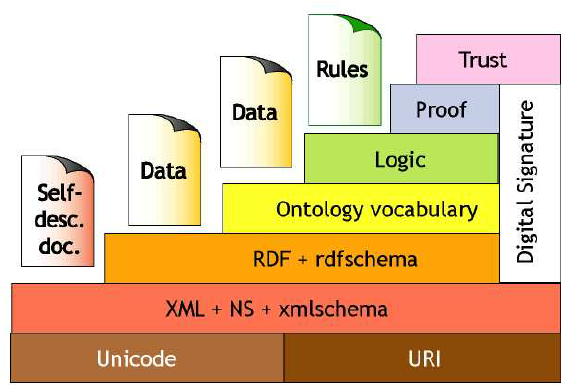
\includegraphics[width=0.7\textwidth]{layered_architecture.png} \label{fig:layered}
	\caption{Arhitectura stratificat\u a pentru semantic web \protect\footnotemark}
\end{figure}

\footnotetext{\url{https://benchpartner.com/explain-semantic-web-layer-approach-stack-tower-with-example}}

\textbf{Caracteristici:}
\begin{itemize}
	\item SaaS business model
	\item Platform\u a software open source
	\item Personalizarea aplica\c tiilor pentru utilizatori
	\item Pooling de resurse
	\item Web inteligent
\end{itemize}


\textbf{Provoc\u ari:}
\begin{itemize}
	\item \emph{Vastitate} - con\c tine miliarde de pagini, ce duce la redundan\c ta datelor
	\item \emph{Vaguitatea} - interog\u arile inprecise de c\u atre utilizatori, precum \c si modul \^in care furnizorii de con\c tinut reprezint\u a conceptele pot face dificil\u a potrivirea termenilor de interogare cu termenii relevan\c ti ai furnizorului. Acest lucru poate fi \c si mai agravat atunci c\^and se \^incearc\u a integrarea mai multor baze de cuno\c stin\c te, care pot de\c tine concepte similare, dar nu identice, ce poate rezulta \^in ambiguitate \c si incertitudine
	\item \emph{Incoeren\c ta} - contradic\c tii logice ce vor ap\u area inevitabil
	\item \emph{\^In\c sel\u aciune} - momentul \^in care sursa de informa\c tii induce \^in eroare inten\c tionat consumatorul de informa\c tii
\end{itemize}

% \newpage
\section{Evolu\c tia tehnologiilor}

Pe m\u asur\u a ce dezvoltarea aplica\c tiilor evolua, la fel au evoluat \c si tehnologiile utilizate \^in crearea aplica\c tiilor. De-a lungul anilor au ap\u arut multe tehnologii care au revolu\c tionat modul \^in care sunt dezvoltate aplica\c tiile. Pe m\u asur\u a ce acestea deveneau mai complexe, necesitatea \^in tehnologii mai performante a devenit evident\u a. La mijlocul anilor 2000 a fost introdus AJAX (\emph{Asynchronus JavaScript and XML}), care a permis aplica\c tiilor web s\u a comunice cu serverele, f\u ar\u a a re\^inc\u arca \^intreaga pagin\u a. Acest lucru a rezultat \^in aplica\c tii web mai rapide \c si receptive. \cite{ajax}

\^In ultimii ani, au ap\u arut mai multe framework-uri front-end, care au facilitat crearea aplica\c tiilor web cu o complexitate sporit\u a. React, Vue, Next, Angular au devenit extrem de populare datorit\u a u\c surin\c tei de utilizare \c si capacit\u a\c tii lor de a gestiona cantit\u a\c ti mari de date. Aceste framework-uri au f\u acut posibil\u a crearea unor aplica\c tii cu un user experience \c si func\c tionalit\u a\c ti ce nu au fost posibile anterior.

Pe l\^ang\u a framework-urile front-end, au evoluat \c si tehnologiile back-end, \^in mod semnificativ. PHP, Ruby on Rails, Node.js au facilitat crearea aplica\c tiilor web moderne scalabile, care pot gestiona cantit\u a\c ti mari de trafic \^in timp real \c si sarcini complexe de procesare a datelor.

Evolu\c tia tehnologiilor web a fost determinat\u a de necesitatea de a crea aplica\c tii mai complexe, cu func\c tionalit\u a\c ti avansate. De la HTML "curat" la framework-uri pentru front-end \c si back-end, tehnologiile web continu\u a s\u a evolueze \^intr-un ritm rapid, fapt ce impune dezvoltatorii s\u a fie la curent cu ultimele tehnologii \c si constant s\u a-\c si actualizeze metodele de dezvoltare utilizate, pentru a deveni mai efectivi \^in dezvoltarea aplica\c tiilor moderne, care r\u aspund nevoilor sporite ale utilizatorilor.

\begin{figure}[htbp]
	\centering
	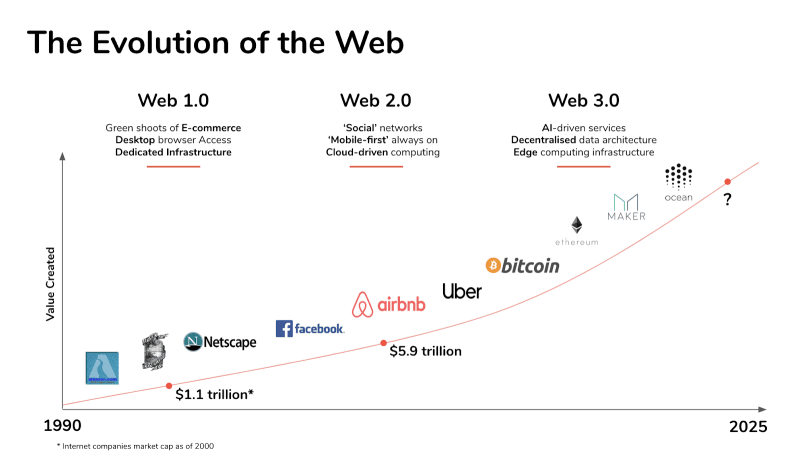
\includegraphics[width=0.9\textwidth]{web-evolution.png} \label{fig:web-evolution}
	\caption{Evolu\c tia web-ului \protect\footnotemark}
\end{figure}

\footnotetext{\url{https://dev.to/pragativerma18/evolution-of-web-42eh}}

Evolutia web a avut un impact semnificativ asupra dezvolt\u arii aplica\c tiilor web moderne. Cre\c sterea vitezei de conectare la internet \c si a performan\c tei dispozitivelor a permis dezvoltarea aplica\c tiilor web complexe, cu func\c tii avansate \c si user experience sporit. Utilizarea extinsa a standardelor web deschise, cum ar fi HTML, CSS \c si JavaScript, a dus la o mai mare interoperabilitate \^intre diferite platforme \c si la o mai mare eficien\c t\u a \^in dezvoltarea aplica\c tiilor.

Apari\c tia \c si popularizarea API-urilor \c si a arhitecturilor RESTful au f\u acut posibil\u a integrarea mai u\c soar\u a a aplicatiilor web cu alte aplica\c tii \c si servicii. Cloud computing-ul \c si serviciile web, cum ar fi Amazon Web Services \c si Microsoft Azure, au f\u acut posibil\u a scalabilitatea \c si distribuirea aplica\c tiilor web cu usurin\c t\u a, indiferent de loca\c tia utilizatorilor.

Cre\c sterea numarului de utilizatori \c si a numarului de dispozitive conectate a dus la o cre\c stere semnificativ\u a a cerin\c telor de securitate \c si a necesit\u a\c tii de a dezvolta aplica\c tii web sigure.

Dezvoltarea \c si popularizarea framework-urilor \c si bibliotecilor de cod, cum ar fi Angular, React \c si Vue, a simplificat dezvoltarea aplica\c tiilor web \c si a \^imbunat\u a\c tit productivitatea dezvoltatorilor.

Aplica\c tiile web moderne sunt mult mai complexe \c si pot include o varietate de componente, cum ar fi front-end, back-end, baze de date, API-uri \c si multe altele. \^In plus, aplica\c tiile web trebuie s\u a functioneze pe o varietate de platforme \c si dispozitive, ceea ce adaug\u a o alt\u a dimensiune a complexit\u a\c tii.

Pe masur\u a ce aplica\c tiile web devin mai complexe, devin mai dificil de dezvoltat \c si de \^intre\c tinut. Dezvolatorii trebuie s\u a se concentreze nu numai pe func\c tionalitatea aplica\c tiei, ci \c si pe asigurarea securit\u a\c tii \c si performan\c tei acesteia. \^In plus, este necesar s\u a se men\c tin\u a un echilibru \^intre user experience, securitate \c si scalabilitatea aplica\c tiei.

Pentru a face fa\c t\u a acestei complexit\u a\c ti, dezvoltatorii utilizeaz\u a framework-uri \c si biblioteci care simplific\u a procesul de dezvoltare \c si permite o gestionare mai bun\u a a complexit\u a\c tii aplica\c tiilor.


\chapter{Paradigmele actuale de randare}
Rendering-ul este procesul de conversie a datelor \^intr-o reprezentare vizual\u a \c si joac\u a un rol esen\c tial \^in aplica\c tiile web, permi\c t\^and furnizarea de con\c tinut dinamic \c si interactiv c\u atre utilizatori.\^In stadiile incipiente ale dezvolt\u arii web-ului, randarea a fost realizat\u a \^in principal pe server. Site-urile web erau construite folosind tehnologii precum PHP sau Java, unde serverul genera con\c tinutul HTML \^in mod dinamic, pe baza solicit\u arilor utilizatorilor. Aceast\u a abordare are un TTFB (Time to first byte) rapid, deoarece serverul poate genera HTML ce poate fi livrat rapid clientului. Dezavantajul acestei paradigme este c\u a nu este la fel de efectiv\u a pentru site-urile web \^ in care datele se schimb\u a des, ci doar pentru site-urile care nu necesit\u a interactivitate complex\u a sau date dinamice. \cite{benefitsserverrendering}

Multe dintre cele mai mari aplica\c tii web din ziua de azi \^ inc\u a folosesc aceast\u a abordare, cum ar fi, de exemplu, amazon.com: de fiecare dat\u a c\^ and face\c ti click pe un link, ob\c tine\c ti o nou\u a pagin\u a generat\u a dinamic de pe serverele lor. \^ In plus, exist\u a multe framework-uri pentru crearea  aplica\c tiilor multi-page, cum ar fi Ruby on Rails, Django \c si Laravel, precum \c si sisteme de gestionare a con\c tinutului, cum ar fi WordPress. 

\section{Starea de art\u a}

Rendering-ul informa\c tiilor a evoluat semnificativ pe parcursul timpului, \^ in conformitate cu evolu\c tia tehnologiilor web \c si a cerin\c telor utilizatorilor.

La \^ inceput, majoritatea con\c tinutului era generat pe server \c si returnat c\u atre browser \^ in form\u a de pagini HTML statice. Cu trecerea timpului, tehnologiile web au evoluat, ceea ce a permis procesarea dinamic\u a a datelor \^in browser prin intermediul script-urilor. Acest lucru a permis dezvoltarea de aplica\c tii web cu interac\c tiuni complexe \c si randare dinamic\u a a con\c tinutului. Cu toate acestea, performan\c ta aplica\c tiilor web bazate exclusiv pe randare client-side a putut fi limitat\u a \^ in condi\c tii de conexiune lent\u a la internet. Din acest motiv, tehnologiile de randare hibrid\u a au devenit din ce \^ in ce mai populare, combin\^ and avantajele rand\u arii server-side \c si client-side. \cite{html}

\^ In prezent, tehnologiile de randare se bazeaz\u a pe framework-uri \c si biblioteci moderne, cum ar fi React, Angular \c si Vue, care ofer\u a unelte puternice pentru a construi aplica\c tii web performante \c si cu o experien\c t\u a utilizator remarcabil\u a. \^ In plus, tehnologiile de randare moderne permit integrarea cu alte tehnologii precum WebAssembly \c si Web Workers, care au ca scop \^ imbun\u at\u a\c tirea performan\c tei aplica\c tiilor web. De asemenea, tehnologiile de randare permit utilizarea de anima\c tii \c si interac\c tiuni complexe, care rezult\u a \^intr-un user experience sporit al aplica\c tiei.

Evolu\c tia tehnologiei web \c si a cerin\c telor utilizatorilor continu\u a, iar randarea informa\c tiilor este un domeniu \^ in continu\u a schimbare \c si dezvoltare. \^ In etapa curent\u a de dezvoltare a aplica\c tiilor web, predomin\u a utilizarea larg\u a a JavaScript \c si bibliotecilor JavaScript, cum ar fi React \c si Vue.js.

React, dezvoltat de Facebook, a devenit una dintre tehnologiile cele mai populare pentru construirea de aplica\c tii web, datorit\u a abilit\u a\c tii sale de a oferi o experien\c t\u a de randare eficient\u a \c si de \^ inalt\u a performan\c t\u a. Vue.js, dezvoltat de comunitate, se concentreaz\u a pe simplitate \c si u\c surin\c t\u a de utilizare, fiind o alegere popular\u a pentru proiecte mai mici sau pentru dezvoltatorii care \^ incearc\u a s\u a \^ inve\c te tehnologii moderne de randare a informa\c tiilor.

Exist\u a mai multe tipuri de randare a con\c tinutului, cele mai populare fiind randarea \emph{server-side}, \emph{client-side} \c si  \emph{static server generation}: \cite{clientsidevssercerside}
\begin{enumerate}
	\item \textbf{Server-side rendering:} Procesarea datelor \c si generarea HTML se realizeaz\u a pe server. Server-ul returneaz\u a apoi HTML-ul generat c\u atre browser, care \^il afi\c seaz\u a utilizatorului. Aceast\u a metod\u a de randare este utilizat\u a \^in mod traditional \^in aplica\c tiile web vechi. Avantajul acestei metode este c\u a se poate efectua o procesare a datelor pe server \c si se poate oferi o experien\c t\u a utilizator consistent\u a chiar \c si \^in condi\c tii de conexiune lent\u a la internet. Afi\c sarea ini\c tial\u a a paginii poate fi rapid\u a deoarece clientul nu trebuie s\u a a\c stepte \^inc\u arcarea sau executarea JavaScript-ului \^inainte de afi\c sarea con\c tinutului.
	\item \textbf{Client-side rendering:} Browser-ul prime\c ste date brute \c si le proceseaz\u a prin intermediul unui script (cum ar fi JavaScript) pentru a genera HTML. Aceast\u a metod\u a de randare permite o flexibilitate mai mare \^in prezentarea con\c tinutului \c si ofer\u a posibilitatea de a construi interac\c tiuni complexe cu utilizatorul, cum ar fi formulare dinamice \c si componente grafice interactive. Dezavantajul acestei metode este c\u a necesit\u a mai mult\u a putere de procesare a clientului \c si poate fi mai pu\c tin performant\u a \^in condi\c tii de conexiune lent\u a la internet, deoarece clientul trebuie s\u a a\c stepte desc\u arcarea scripturilor \c si a datelor necesare \^inainte de a randa pagina.
	\item \textbf{Static server generation:} Paginile web sunt pregenerate \c si randate \^in timpul procesului de build al aplica\c tiei, rezult\^and \^in fi\c siere HTML statice care pot fi furnizate c\u atre client f\u ar\u a a fi necesar\u a procesarea la nivelul serverului. Cu SSG, con\c tinutul r\u am\^ane static p\^an\u a la urm\u atorul build al aplica\c tiei.
\end{enumerate}

\^ In ceea ce prive\c ste performan\c ta, tehnologiile moderne de randare a informa\c tiilor au avansat mult \^ in optimizarea vitezei de randare \c si a eficien\c tei resurselor. Una dintre abord\u arile moderne de optimizare a performan\c tei este utilizarea \emph{"virtual DOM"} (Document Object Model), care se caracterizeaz\u a printr-o rerandare eficient\u a doar a componentelor ce au suferit modific\u ari.
\^ In plus, tehnologiile de randare moderne pot delimita componentele dinamice, care necesit\u a rerandare constant\u a, de cele statice, care nu necesit\u a recalculare, cresc\^ and astfel performan\c ta aplica\c tiei. De asemenea, tehnologiile de randare permit utilizarea de tehnici de lazy loading, care \^ incarc\u a con\c tinutul doar atunci c\^ and este necesar, \^ imbun\u at\u a\c tind astfel performan\c ta aplica\c tiei \c si experien\c ta utilizatorului. \cite{virtual-dom}
Alegerea metodei potrivite de randare depinde de cerin\c tele specifice ale proiectului \c si poate include considera\c tii legate de performan\c ta, flexibilitatea \c si compatibilitatea cu echipamentele utilizatorilor. Este important s\u a se \^ in\c teleag\u a avantajele \c si dezavantajele fiec\u arei metode \c si s\u a se fac\u a o evaluare corespunz\u atoare a acestora \^ inainte de a lua o decizie.


\section{Client side rendering}

Re\^ inc\u arcarea \^ intregii pagini la fiecare schimbare de URL este un proces costisitor, de aceea pentru a reduce necesitatea de a regenera con\c tinutul au ap\u arut solu\c tii precum React \c si Angular - framework-uri JavaScript, ce permit modificarea componentelor f\u ar\u a a cauza o re\^ inc\u arcare a paginii. Aceast\u a arhitectur\u a se nume\c ste SPA (\textit{Single Page Application}).

\^Intr-un SPA, resursele HTML, CSS \c si JavaScript ini\c tiale sunt \^inc\u arcate atunci c\^and aplica\c tia este accesat\u a pentru prima dat\u a. Interac\c tiunile ulterioare \c si modific\u arile st\u arii aplica\c tiei sunt gestionate prin efectuarea de cereri asincrone c\u atre server pentru a ob\c tine date, care sunt apoi randate pe partea de client (\textit{client-side rendering}). Aceasta rezult\u a \^intr-o experien\c t\u a mai receptiv\u a \c si interactiv\u a, deoarece aplica\c tia poate actualiza componente sau sec\c tiuni specifice ale paginii f\u ar\u a a comunica cu serverul.

O aplica\c tie ce utilizeaz\u a CSR este caracterizat\u a prin urm\u atoarele aspecte:
\begin{enumerate}
	\item \textbf{Cererea HTTP a clientului} - c\^and utilizatorul introduce URL-ul \^in bara de adrese a browserului, se stabile\c ste o conexiune HTTP cu serverul.
	\item \textbf{R\u aspunsul HTTP al serverului} - Serverul trimite \^inapoi fi\c sierul HTML ini\c tial, care con\c tine referin\c te c\u atre fi\c siere JavaScript \c si CSS.
	\item \textbf{\^Inc\u arcarea paginii} - browserul clientului prime\c ste fi\c sierul HTML ini\c tial \c si \^incepe randarea structurii de baz\u a a paginii, inclusiv orice con\c tinut static.
	\item \textbf{\^Inc\u arcarea fi\c sierelor JavaScript} - browserul descarc\u a fi\c sierele JavaScript referen\c tiate \^in fi\c sierul HTML ini\c tial.
	\item \textbf{Preluarea datelor} - codul JavaScript executat de browserul clientului face cereri c\u atre server sau API-uri, pentru a prelua datele necesare pentru a randa con\c tinutul dinamic.
	\item \textbf{Randarea \c si actualizarea} - odat\u a ce datele sunt preluate, codul JavaScript proceseaz\u a datele \c si genereaz\u a dinamic structura HTML necesar\u a. Browserul actualizeaz\u a pagina randat\u a cu con\c tinutul HTML generat dinamic, care poate include liste, tabele, formulare sau alte componente
	\item \textbf{Interactivitatea} - ascult\u atorii de evenimente \c si interac\c tiunile utilizatorului, cum ar fi click-urile sau introducerile de date, declan\c seaz\u a execu\c tia de cod JavaScript ulterioar\u a, care poate actualiza con\c tinutul randat, f\u ar\u a a necesita o re\^inc\u arcare complet\u a a paginii.
\end{enumerate}
\newpage
\begin{figure}[htbp]
	\centering
	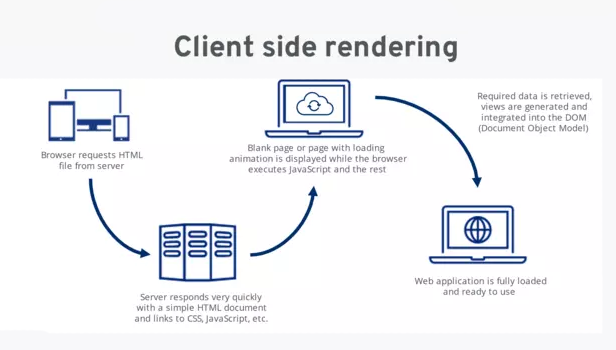
\includegraphics[width=0.9\textwidth]{csr-diagram.png}
	\caption{Client side rendering \protect\footnotemark}
	\label{fig:csr-diagram}
\end{figure}

\footnotetext{\url{https://www.ionos.ca/digitalguide/websites/web-development/server-side-and-client-side-scripting-the-differences/}}

Deoarece browserul trebuie s\u a descarce \c si s\u a ruleze \^intregul cod al aplica\c tiei \^inainte ca con\c tinutul s\u a apar\u a pe ecran, \^inc\u arcarea ini\c tial\u a a paginii este de obicei lent\u a. Ca rezultat, utilizatorii v\u ad o pagin\u a goal\u a sau un indicator de \^inc\u arcare pentru o perioad\u a relativ lung\u a de timp. Aceasta duce la o experien\c t\u a mai pu\c tin pl\u acut\u a pentru utilizatori \c si la o rat\u a mai mare de abandon\u ari a paginii (\textit{bounce rate}). \cite{google-bouncing-rate}

Cu toate acestea, pot exista provoc\u ari \^in ceea ce prive\c ste optimizarea pentru motoarele de c\u autare (SEO), deoarece toate resursele aplica\c tiei sunt \^inc\u arcate la prima accesare, crawler-ii web tradi\c tionali pot \^int\^ampina dificult\u a\c ti \^in parcurgerea \c si indexarea con\c tinutului, iar volumul mare de scripturi ce sunt desc\u arcate, bibliotecile externe \c si dependen\c tele pot rezulta \^intr-un timp de \^inc\u arcare ini\c tial mai mare.

\section{Server side rendering}

O nou\u a abordare, ce avea scopul de a rezolva problemele aplicatiilor single page este server-side rendering (SSR).

SSR este o tehnic\u a \^in dezvoltarea aplica\c tiilor web care implic\u a generarea de HTML pe server \c si trimiterea acestuia c\u atre client. Spre deosebire de CSR, procesul de randare se execut\u a pe server, ce reprezint\u a un avantaj semnificativ, datorit\u a timpului mai rapid de \^inc\u arcare ini\c tial\u a a paginilor. \cite{benefitsserverrendering}

\begin{figure}[htbp]
	\centering
	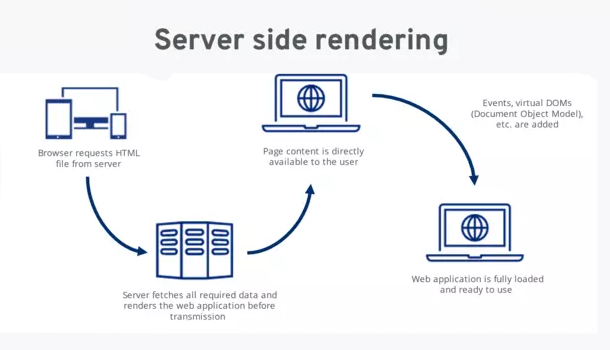
\includegraphics[width=0.9\textwidth]{ssr-diagram.png}
	\caption{Server side rendering \protect\footnotemark}
	\label{fig:ssr-diagram}
\end{figure}

\footnotetext{\url{https://www.ionos.ca/digitalguide/websites/web-development/server-side-and-client-side-scripting-the-differences/}}

Un alt avantaj al SSR este \^imbun\u at\u a\c tirea optimiz\u arii pentru motoarele de c\u autare (SEO). Deoarece crawler-ii motoarelor de c\u autare se bazeaz\u a \^in mod tipic pe con\c tinutul HTML, serve-side rendering furnizeaz\u a pagini complet randate motoarelor de c\u autare, care pot fi indexate u\c sor. Aceasta \^imbun\u at\u a\c te\c ste vizibilitatea \c si accesibilitatea site-ului \^in rezultatele motoarelor de c\u autare.

SSR aduce beneficii \c si utilizatorilor cu conexiuni lente la internet sau dispozitive mai vechi. Prin pre-randarea HTML-ului pe server, SSR asigur\u a utilizatorii cu con\c tinut chiar \c si \^in cazul \^in care dispozitivele lor au putere de procesare limitat\u a sau capacit\u a\c ti de re\c tea reduse. Aceasta \^imbun\u at\u a\c te\c ste accesibilitatea \c si experien\c ta utilizatorului pentru o gam\u a mai larg\u a de utilizatori.

Server-side rendering are c\^ateva dezavantaje asociate. Deoarece fiecare solicitare necesit\u a o nou\u a randare pe server, aceasta poate duce la o \^inc\u arcare mai mare a serverului \c si la un timp de r\u aspuns mai lent. De asemenea, este mai dificil de implementat \c si de \^intre\c tinut, deoarece necesit\u a o infrastructur\u a de servere mai complex\u a. SSR creeaz\u a o dependen\c t\u a de server, deoarece clientul prime\c ste pagini complet redat\u a de la server. \^In cazul \^in care serverul \^int\^ampin\u a probleme sau este indisponibil, utilizatorii nu pot accesa sau utiliza aplica\c tia.
Gestionarea st\u arii clientului poate deveni \c si mai complex\u a cu SSR. Sincronizarea \c si actualizarea st\u arii \^intre client \c si server pentru a men\c tine coeren\c ta aplica\c tiei necesit\u a o implementare bine g\^andit\u a \c si poate fi dificil de gestionat.

O aplica\c tie ce utilizeaz\u a SSR este caracterizat\u a prin urm\u atoarele aspecte:

\begin{enumerate}
	\item \textbf{Cererea HTTP din partea clientului} - c\^and utlizitorul introduce URL-ul \^in broswer, se stabile\c ste o conexiune HTTP cu serverul \c si apoi se trimite serverului o cerere pentru a ob\c tine documentul HTML.
	\item \textbf{Preluarea datelor} - serverul preia datele necesare din baza de date sau API-uri.
	\item \textbf{Pre-randarea pe partea de server} - serverul compileaz\u a componentele JavaScript \^in HTML static.
	\item \textbf{R\u aspunsul HTTP al serverului} - serverul trimite documentul compilat c\u atre client.
	\item \textbf{\^Inc\u arcarea \c si afi\c sarea paginii} - clientul descarc\u a fi\c sierul HTML \c si afi\c seaz\u a componentele statice pe pagin\u a.
	\item \textbf{Hidratarea} - clientul descarc\u a fi\c sierul sau fi\c sierele JavaScript \^incorporate \^in HTML, proceseaz\u a codul \c si ata\c seaz\u a ascult\u atori de evenimente componentelor.
\end{enumerate} \cite{improve-ssr-speed}

\section{Static server generation}

SSG este o paradigma alternativ\u a \^in dezvoltarea web care \^imbin\u a beneficiile SSR \c si CSR. Spre deosebire de server-side rendering, unde HTML-ul este generat dinamic la fiecare cerere, SSG genereaz\u a fi\c siere HTML statice \^in timpul procesului de build, care sunt apoi servite c\u atre client.

Unul dintre avantajele majore ale SSG este performan\c ta \^imbun\u at\u a\c tit\u a \c si scalabilitatea. Deoarece HTML-ul este pre-randat, serverul poate servi fi\c siere statice direct, f\u ar\u a a necesita prelucr\u ari suplimentare. Aceasta duce la \^inc\u arcarea mai rapid\u a a paginilor \c si reducerea \^inc\u arc\u arii serverului, f\u ac\^andu-l potrivit pentru site-urile cu trafic intens. 

\begin{figure}[htbp]
	\centering
	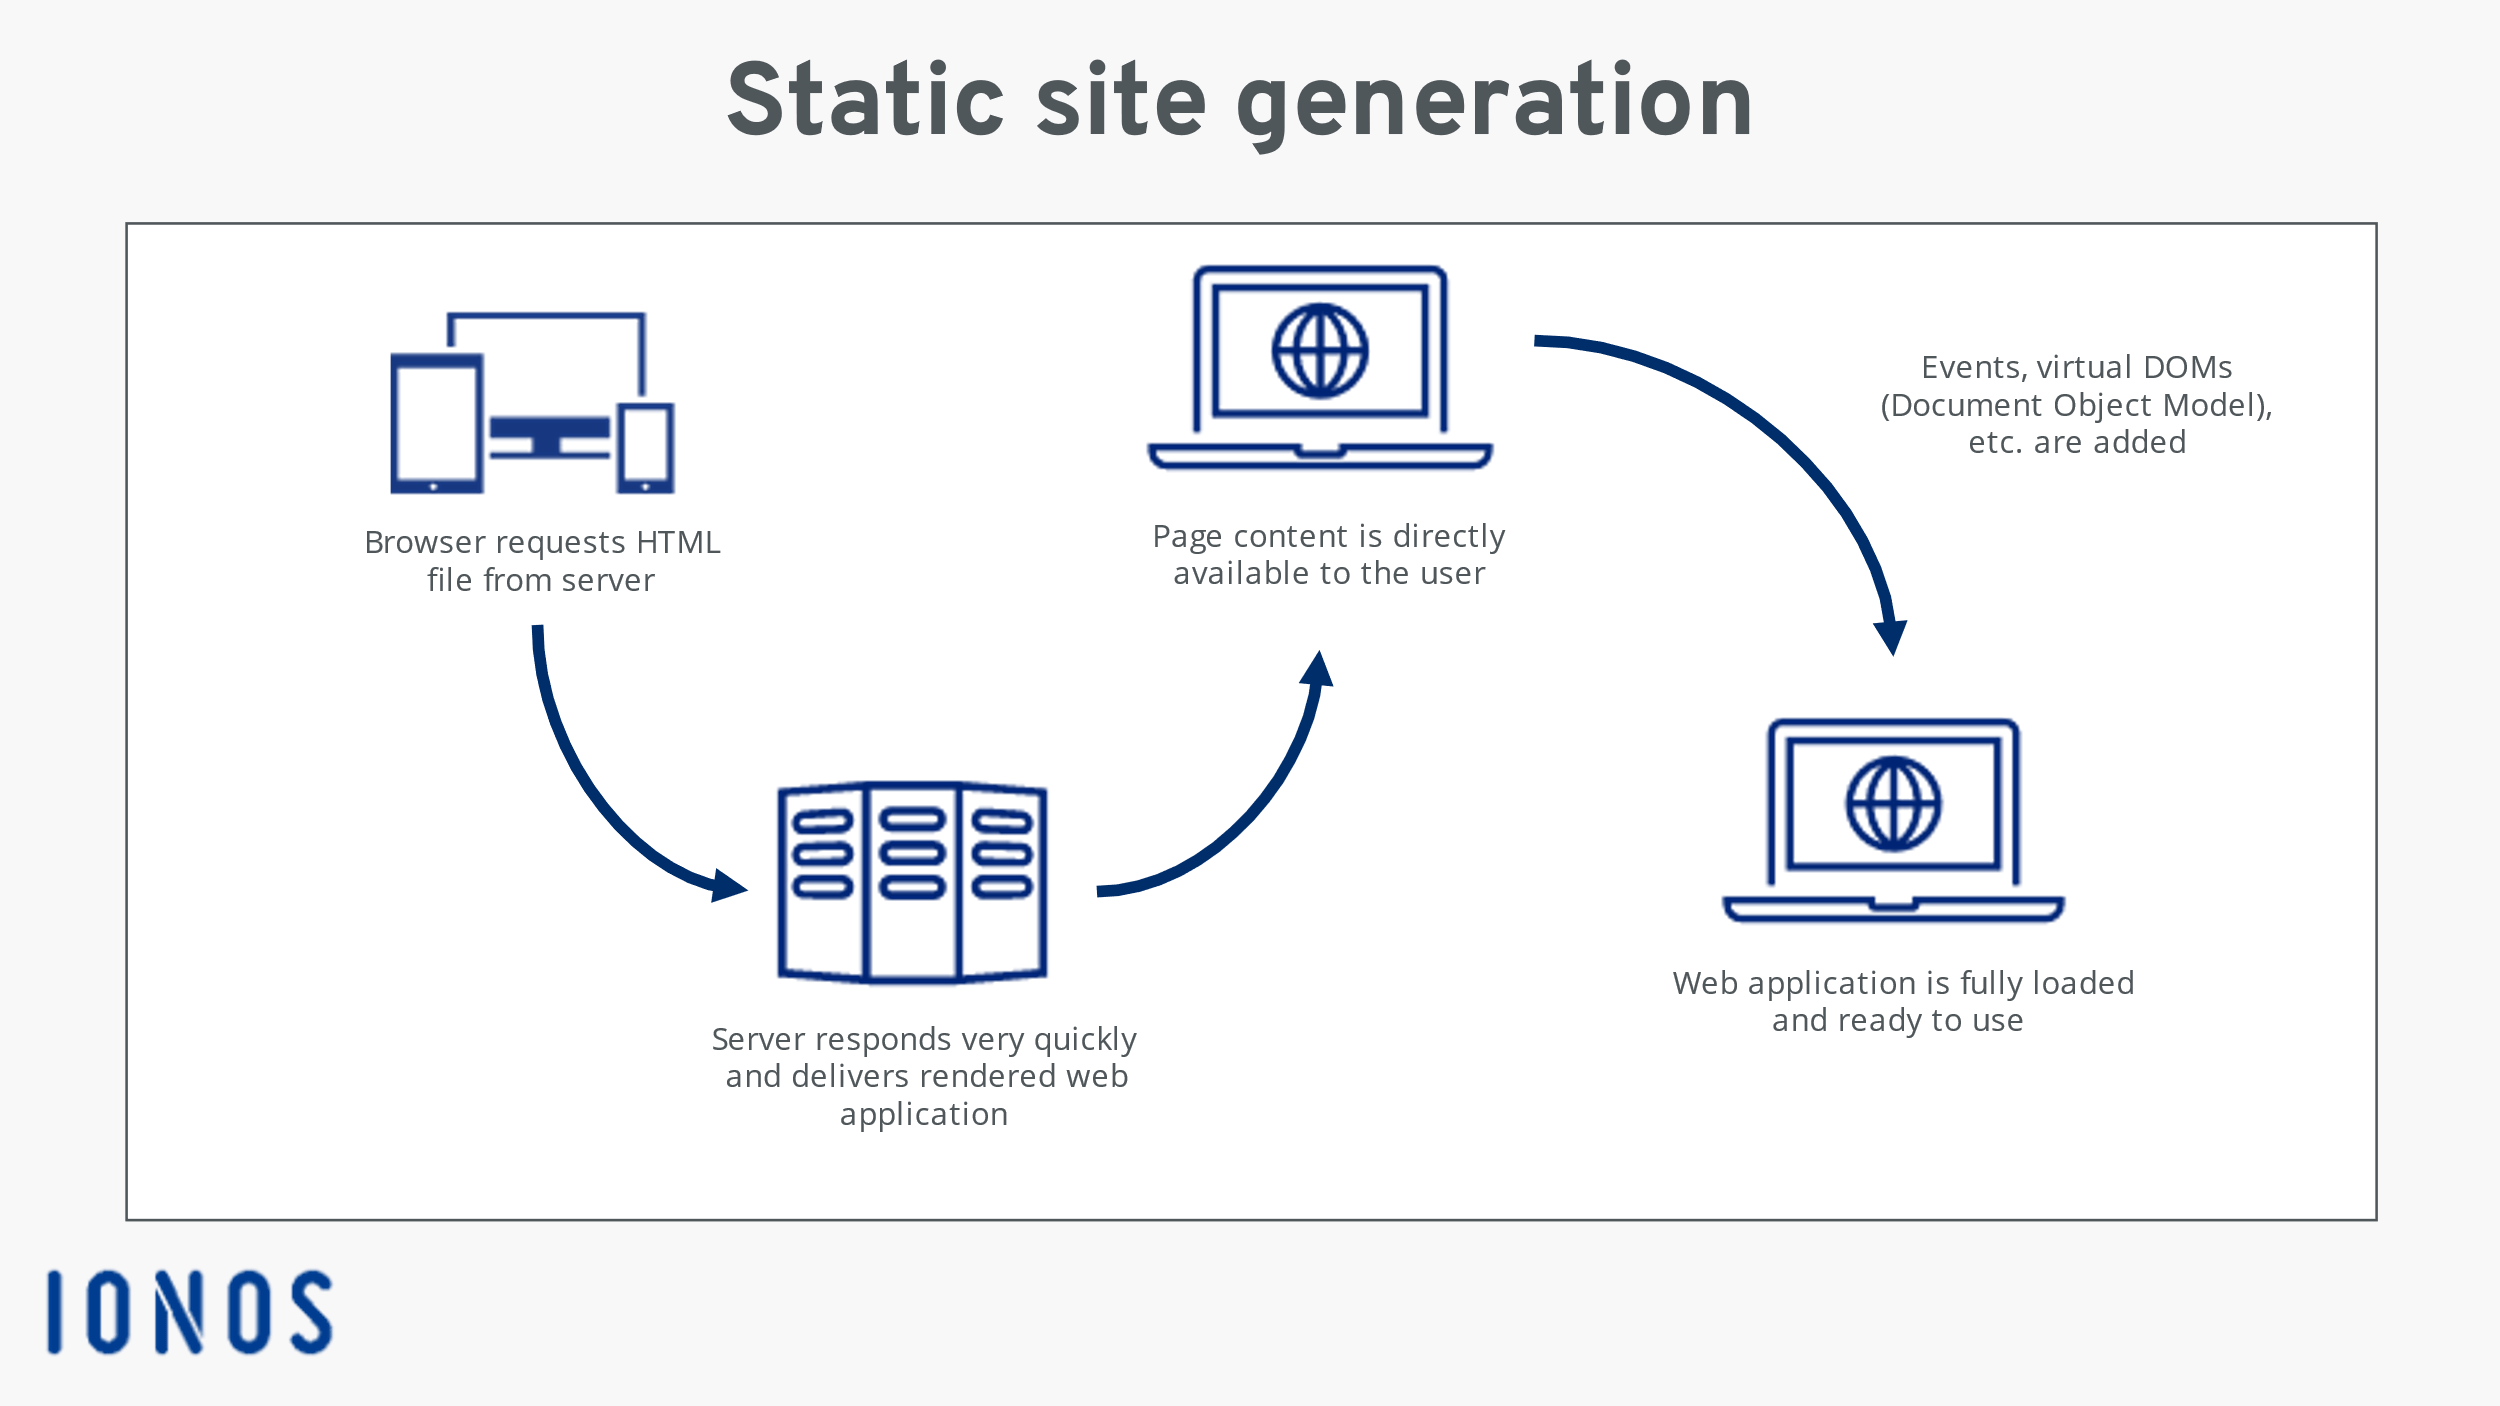
\includegraphics[width=0.8\textwidth]{ssg-diagram.png}
	\caption{Static server generation \protect\footnotemark}
	\label{fig:ssg}
\end{figure}
\footnotetext{\url{https://www.ionos.ca/digitalguide/websites/web-development/server-side-and-client-side-scripting-the-differences/}}


O aplica\c tie ce utilizeaz\u a SSR este caracterizat\u a prin urm\u atoarele aspecte:
\begin{enumerate}
	\item \textbf{Procesul de build} - \^in timpul acestui proces codul surs\u a \c si fi\c sierele de con\c tinut ale site-ului web sunt analizate.
	\item \textbf{Compilarea con\c tinutului} - con\c tinutul fi\c sierelor este procesat \c si convertit din formatul surs\u a (Markdown sau YAML) \^in formatul HTML.
	\item \textbf{Modelarea} - sunt aplicate \c sabloane pe fi\c sierele compilate, permi\c t\^and un aspect \c si o structur\u a coerent\u a.
	\item \textbf{Integrarea datelor} - sunt preluate date din diverse surse (baze de date, API-uri) \c si sunt integrate \^in paginile generate anterior.
	\item \textbf{Generarea HTML-ului static} - fi\c sierele HTML sunt generate pe baza con\c tinutului compilat, a \c sabloanelor \c si a datelor integrate.
	\item \textbf{Optimizarea resurselor} - \^in timpul procesului de build, resursele precum CSS, JavaScript \c si imaginile se optimizeaz\u a, reduc\^and dimensiunile fi\c sierelor \c si \^imbun\u at\u a\c tind performan\c ta.
	\item \textbf{Implementarea} -  odat\u a ce fi\c sierele statice sunt generate, acestea pot fi p\u astrate \^in cache pe server sau pe CDN, permi\c t\^and servirea instantanee a cererilor ulterioare f\u ar\u a a necesita regenerarea lor (\textit{minimizeaz\u a \^inc\u arcarea serverului \c si \^imbun\u at\u a\c te\c ste scalabilitatea general\u a, \^in special \^in scenarii \^in care actualiz\u arile de con\c tinut sunt rare}).
	\item \textbf{Cererea clientului} -  c\^and un utilizator viziteaz\u a o pagin\u a, serverul web sau CDN-ul serve\c ste direct fi\c sierul HTML static pre-generat.
	\item \textbf{Afi\c sarea paginii} - browserul clientului prime\c ste fi\c sierul HTML static \c si afi\c seaz\u a con\c tinutul pe pagin\u a.
	\item \textbf{Interactivitatea} - Dac\u a exist\u a elemente interactive sau func\c tionalit\u a\c ti dinamice pe pagin\u a, codul JavaScript poate fi utilizat pentru a \^imbun\u at\u a\c ti experien\c ta utilizatorului, de obicei prin preluarea de date suplimentare din API-uri sau prin gestionarea interac\c tiunilor utilizatorului.
\end{enumerate}

Cu toate acestea are \c si c\^ateva limit\u ari. SSG nu este potrivit pentru aplica\c tii ce necesit\u a actualiz\u ari \^in timp real sau con\c tinut dinamic, deoarece fi\c sierele statice pre-randate nu se modific\u a p\^an\u a la urm\u atorul proces de build. Acest lucru poate introduce \^int\^arzieri \^in disponibilitatea con\c tinutului \c si cre\c sterea complexit\u a\c tii gestion\u arii actualiz\u arilor de con\c tinut. \cite{rendering-patterns}
Unul dintre cele mai mari dezavantaje ale acestui abord\u ari este timpul de build. Dac\u a site-ul cons\u a dintr-un num\u ar mare de pagini, procesul de build al acestora va dura mult timp.


\section{Alegerea paradigmei corespunz\u atoare}

Alegerea \^intre CSR, SSR \c si SSG este important\u a \^in dezvoltarea unei aplica\c tii web, deoarece are un impact direct asupra experien\c tei utilizatorului, performan\c tei \c si func\c tionalit\u a\c tii generale a aplica\c tiei. Fiecare abordare are propriile sale puncte forte \c si considera\c tii, iar alegerea depinde de mai mul\c ti factori, cum ar fi cerin\c tele proiectului, scalabilitatea, complexitatea \c si obiectivele de performan\c t\u a. Principalele aspecte de luat \^in considerare sunt:\cite{choose-rendering}

\begin{enumerate}
	\item \textbf{Experien\c ta utilizatorului} - Abordarea de randare afecteaz\u a \^in mod semnificativ modul \^in care con\c tinutul aplica\c tiei este livrat \^in browserul utilizatorului. CSR pune accent pe interactivitate, prin \^inc\u arcarea ini\c tial\u a a unei structuri HTML minimale \c si apoi preluarea \c si randarea datelor pe partea clientului, ceea ce duce la o \^inc\u arcare ini\c tial\u a mai rapid\u a a paginii. SSR, pe de alt\u a parte, furnizeaz\u a o pagin\u a HTML complet redat\u a de pe server, fapt ce reduce timpul de \^inc\u arcare ini\c tial \c si asigur\u a ca con\c tinutul s\u a fie imediat vizibil utilizatorilor. SSG genereaz\u a fi\c siere HTML statice \^in timpul procesului de construc\c tie, permit\^and \^inc\u arc\u ari de pagini ultra-rapide, deoarece nu este necesar\u a prelucrarea \^in server.
	\item \textbf{Optimizarea pentru motoarele de c\u autare} - Motoarele de c\u autare \^int\^ampin\u a adesea dificult\u a\c ti \^in indexarea con\c tinutului JavaScript dinamic. SSR \c si SSG, care livreaz\u a con\c tinut HTML pre-randat \^in browser, sunt mai efective cu SEO \^in compara\c tie cu CSR. Acest lucru se datoreaz\u a faptului c\u a motoarele de c\u autare pot parcurge \c si indexa u\c sor con\c tinutul HTML static, ceea ce ajut\u a la \^imbun\u at\u a\c tirea vizibilit\u a\c tii \c si descoperirii.
	\item \textbf{Performan\c ta} - Abordarea de randare afecteaz\u a performan\c ta general\u a a aplica\c tiei. CSR poate duce la timp de \^inc\u arcare mai lung, \^in special \^in cazul conexiunilor de re\c tea mai lente sau al unor cantit\u a\c ti mari de date de preluat. SSR reduce timpul de randare ini\c tial prin furnizarea unei pagini pre-randate de pe server, \^ins\u a navigarea ulterioar\u a poate necesita apeluri suplimentare c\u atre server. SSG ofer\u a cea mai bun\u a performan\c t\u a, deoarece genereaz\u a fi\c siere HTML statice care pot fi livrate direct utilizatorului, minimiz\^and necesitatea de prelucrare pe server.
	\item \textbf{Complexitatea \c si fluxul de dezvoltare} - Framework-urile CSR, cum ar fi React, Angular sau Vue.js, necesit\u a ca dezvoltatorii s\u a gestioneze logica de randare \c si st\u ariile componentelor, ceea ce poate introduce complexitate. SSR \c si SSG reduc, \^intr-o anumit\u a m\u asur\u a, aceast\u a complexitate prin transferul logicii de randare la server sau la procesul de build al aplica\c tiei. SSR necesit\u a configurare pe partea de server \c si cuno\c stin\c te despre tehnologiile backend, \^in timp ce SSG simplific\u a fluxul de lucru \^in dezvoltare prin generarea de active statice care pot fi u\c sor implementate pe orice server web.
	\item \textbf{Con\c tinutul dinamic \c si actualiz\u ari \^in timp real} - CSR se eviden\c tiaz\u a \^in aplica\c tiile extrem de interactive care se bazeaz\u a pe actualiz\u ari frecvente ale datelor sau pe func\c tionalit\u a\c ti \^in timp real. Cu CSR, datele pot fi actualizate f\u ar\u a necesitatea unei re\^inc\u arc\u ari complete a paginii. SSR \c si SSG sunt mai potrivite pentru aplica\c tiile axate pe con\c tinut mai pu\c tin dinamic, deoarece necesit\u a o solicitare c\u atre server pentru a actualiza datele.
\end{enumerate}

Alegerea paradigmei potrivite este esen\c tial\u a pentru a furniza o aplica\c tie web rapid\u a, interactiv\u a \c si optimizat\u a pentru motoarele de c\u autare. De asemenea, este important s\u a se ia \^in considerare cerin\c tele proiectului, complexitatea \c si obiectivele de performan\c t\u a pentru a determina cea mai bun\u a abordare de randare. Aceasta este una dintre primele decizii importante ce trebuie luat\u a \^in dezvoltarea unei aplica\c tii web, deoarece este dificil de schimbat ulterior.

\chapter{Aplica\c tia practic\u a}

Obiectivul acestui capitol este de a oferi o experien\c t\u a practic\u a cu tehnologiile de randare \c si de a evalua performan\c ta \c si eficien\c ta acestora. Rezultatele ob\c tinute vor fi valoroase pentru dezvoltatori \c si arhitec\c ti care doresc s\u a optimizeze procesele de randare \c si s\u a \^imbun\u at\u a\c teasc\u a experien\c ta utilizatorului.

% Pentru obiectivitatea experimentului, a fost implementa aceea\c si aplica\c tie cu ajutorul la mai multe framework-uri JavaScript, c\^at \c si \^in vanilla (\emph{plain}) JavaScript, pentru a ob\c tine rezultate ce se vor putea compara, pentru a identifica cele mai optime abordari posibile.

Pentru o obiectivitate sporit\u a a fost implementat\u a aceea\c si aplica\c tie, cu ajutorul mai multor framework-uri JavaScript, fiecare dintre ele reprezent\^and o abordare diferit\u a de randare (CSR, SSR, SSG). De asemenea, aplica\c tia a fost implementat\u a \c si cu ajutorul vanilla JavaScript, pentru a compara aplica\c tiile dup\u a un anumit set de criterii cu scopul de a identifica care sunt aspectele cheie care difer\u a \^intre aplica\c tiile construite cu ajutorul framework-urilor JavaScript \c si cea construit\u a folosind vanilla JavaScript. Rezultatul acestui studiu comparativ ofer\u a o imagine de ansamblu asupra avantajelor \c si dezavantajelor fiec\u arei tehnici de randare, precum \c si a celor mai optime abord\u ari posibile.


\section{Metrici de performan\c t\u a}

Pentru compararea efectiv\u a a metodelor de implementare, este nevoie de a compara rezultatele dup\u a anumite criterii care reprezint\u a performan\c ta general\u a a aplica\c tiei.
Metricile care vor fi utilizate \^in evaluarea performan\c tei pentru toate implement\u arile sunt:

\begin{itemize}
	\item \textbf{Largest Contentful Paint (\emph{LCP})} - metric\u a de performan\c t\u a utilizat\u a pentru a m\u asura viteza de \^inc\u arcare \c si stabilitatea vizual\u a perceput\u a a unei pagini web, introdus\u a de Google. LCP m\u asoar\u a timpul necesar ca cel mai mare element vizibil de pe o pagin\u a web s\u a fie afi\c sat \^in zona de vizualizare a utilizatorului. Acest element poate fi o imagine, un videoclip sau un element de tip block, cum ar fi un paragraf sau un antet. Cu c\^at LCP este mai rapid, cu at\^at este mai bun\u a experien\c ta utilizatorului, deoarece indic\u a faptul c\u a con\c tinutul principal al paginii este afi\c sat rapid. Un scor bun al LCP este considerat \^in general sub 2,5 secunde. Dac\u a LCP dep\u a\c se\c ste acest prag, poate duce la o rat\u a mai mare de respingere \c si poate afecta negativ angajamentul utilizatorului. Pentru a \^imbun\u at\u a\c ti LCP, dezvoltatorii web pot optimiza performan\c ta site-ului prin minimizarea resurselor care blocheaz\u a afi\c sarea, optimizarea imaginilor \c si videoclipurilor \c si implementarea tehnicilor precum lazy-load \c si code splitting.

	      LCP este una dintre principalele metrici luate \^in considerare de motoarele de c\u autare, inclusiv Google, pentru a evalua experien\c ta utilizatorului pe un site web. Site-urile cu scoruri bune ale LCP sunt mai susceptibile de a ob\c tine un rang mai \^inalt \^in rezultatele c\u aut\u arii \c si de a oferi o experien\c t\u a de navigare mai bun\u a utilizatorilor. \cite{lcp}
	\item \textbf{Cumulative Layout Shift (\emph{CLS})} - este utilizat\u a pentru a m\u asura stabilitatea vizual\u a a unei pagini web. Aceasta cuantific\u a cantitatea de schimb\u ari de aspect nea\c steptate care apar \^in timpul \^inc\u arc\u arii paginii. Schimbarea de aspect se refer\u a la mi\c scarea elementelor paginii, cum ar fi imagini, butoane sau text, \^intr-un mod care perturb\u a experien\c ta de citire sau de interac\c tiune a utilizatorului. Aceste schimb\u ari pot fi frustrante pentru utilizatori, \^in special atunci c\^and cauzeaz\u a click-uri accidentale sau fac con\c tinutul dificil de citit.

	      CLS este calculat prin m\u asurarea frac\c tiunii de impact \c si frac\c tiunii de distan\c t\u a a fiec\u arui eveniment de schimbare de aspect \c si apoi \^insum\^andu-le pe \^intreaga \^inc\u arcare a paginii. Frac\c tiunea de impact reprezint\u a propor\c tia vizualiz\u arii afectat\u a de schimbare, \^in timp ce frac\c tiunea de distan\c t\u a reprezint\u a distan\c ta maxim\u a pe care elementul o parcurge \^in raport cu ecranul utilizatorului. \cite{cls}

	      Pentru a oferi o bun\u a experien\c t\u a utilizatorului, o pagin\u a web ar trebui s\u a aib\u a un scor CLS sc\u azut. Un scor CLS sub 0.1 este considerat excelent, \^intre 0.1 \c si 0.25 este considerat bun, \^in timp ce scorurile peste 0.25 sunt considerate slabe.

	      Pentru a reduce CLS, dezvoltatorii web pot urma practici, cum ar fi stabilirea dimensiunilor explicite pentru elementele media, rezervarea spa\c tiului pentru reclame sau con\c tinut dinamic \c si evitarea inject\u arii dinamice a con\c tinutului deasupra elementelor existente. Prin minimizarea schimb\u arilor de aspect nea\c steptate, dezvoltatorii pot \^imbun\u at\u a\c ti stabilitatea vizual\u a a paginilor web \c si experien\c ta utilizatorilor.
	\item \textbf{First Input Delay (\emph{FID})} - m\u asoar\u a reactivitatea \c si interactivitatea unei pagini web. Ea cuantific\u a timpul necesar ca o pagin\u a web s\u a r\u aspund\u a la prima interac\c tiune a utilizatorului, cum ar fi ap\u asarea unui buton sau selectarea unui meniu derulant.

	      FID se concentreaz\u a \^in mod specific pe \^int\^arzierea dintre prima interac\c tiune a utilizatorului \c si capacitatea browserului de a r\u aspunde la acea interac\c tiune. Este important\u a deoarece reflect\u a reactivitatea perceput\u a a unui site web \c si are un impact direct asupra experien\c tei utilizatorului. Un FID redus indic\u a un site web mai interactiv \c si mai receptiv, \^in timp ce un FID ridicat poate face un site web s\u a par\u a lent \c si neinteractiv. \cite{fid}

	      FID-ul este m\u asurat \^in milisecunde (ms), iar un scor bun este considerat a fi mai mic de 100 de milisecunde. Un scor peste 300 de milisecunde este considerat slab \c si poate rezulta \^intr-o experien\c t\u a frustrant\u a pentru utilizatori.

	      Pentru a \^imbun\u at\u a\c ti FID, dezvoltatorii web pot optimiza codul lor, reduce timpul de execu\c tie al JavaScript-ului \c si prioritiza sarcinile critice pentru a asigura timp de r\u aspuns mai rapid la interac\c tiunile utilizatorului. Tehnici precum minimizarea codului, \^imp\u ar\c tirea codului \c si \^inc\u arcarea asincron\u a a scripturilor pot contribui la reducerea impactului JavaScript-ului asupra FID-ului.

	      FID-ul este una dintre metricile centrale ale aspectelor vitale ale webului utilizate de motoarele de c\u autare, inclusiv Google, pentru a evalua experien\c ta utilizatorului pe un site web. Site-urile cu scoruri bune de FID au mai multe \c sanse s\u a ob\c tin\u a un rang mai \^inalt \^in rezultatele c\u aut\u arii \c si s\u a ofere o experien\c t\u a de navigare mai fluid\u a \c si mai captivant\u a utilizatorilor.
	\item \textbf{Interaction to Next Paint (\emph{INP})} -  metric\u a a Core Web Vitals, care va \^inlocui First Input Delay (FID) din martie 2024. INP evalueaz\u a reactivitatea folosind date din Event Timing API. Atunci c\^and o interac\c tiune determin\u a ca o pagin\u a s\u a devin\u a neproductiv\u a, aceasta reprezint\u a o experien\c t\u a utilizator slab\u a. INP observ\u a laten\c ta tuturor interac\c tiunilor pe care le-a realizat utilizatorul cu pagina \c si raporteaz\u a o valoare unic\u a sub care au fost toate (sau aproape toate) interac\c tiunile. Un INP sc\u azut \^inseamn\u a c\u a pagina a putut r\u aspunde \^in mod constant \c si rapid tuturor sau unei mari majorit\u a\c ti a interac\c tiunilor utilizatorului.

	      Unele interac\c tiuni vor dura mai mult dec\^at altele, dar \^in special pentru interac\c tiunile complexe, este important s\u a prezenta\c ti un feedback vizual ini\c tial ca indiciu pentru utilizator c\u a se \^int\^ampl\u a ceva \^in background. Timpul p\^an\u a la urm\u atoarea desenare (\emph{paint}) este cea mai timpurie oportunitate pentru a face acest lucru. Prin urmare, inten\c tia INP nu este de a m\u asura toate efectele ulterioare ale interac\c tiunii (cum ar fi fetch-urile \c si actualiz\u arile UI din alte opera\c tii asincrone), ci timpul \^in care urm\u atoarea desenare este blocat\u a. Prin \^int\^arzierea feedbackului vizual, pute\c ti da utilizatorilor impresia c\u a pagina nu r\u aspunde ac\c tiunilor lor. \cite{inp}

	      Scopul INP este de a asigura ca timpul de la ini\c tierea unei interac\c tiuni de c\u atre utilizator p\^an\u a la urm\u atoarea cadru desenat s\u a fie c\^at mai scurt posibil, pentru toate sau majoritatea interac\c tiunilor realizate de utilizator.
\end{itemize}

\section{Metode de evaluare a performan\c tei}

Exist\u a mai multe metode disponibile pentru m\u asurarea performan\c tei unei aplica\c tii web. Aceste instrumente pot ajuta dezvoltatorii s\u a monitorizeze \c si s\u a \^imbun\u at\u a\c teasc\u a performan\c ta \c si experien\c ta utilizatorilor.

\^In evaluarea aplica\c tiei curente au fost folosite urm\u atoarele metode de evaluare a performan\c tei:

\begin{itemize}
	\item  \textbf{Web Vitals} (extensie pentru browser) - ini\c tiativ\u a de la Google, care ofer\u a ghidare unitar\u a pentru semnalele de calitate care sunt esen\c tiale pentru a oferi o experien\c t\u a excelent\u a utilizatorilor pe web.

	      Google a furnizat o serie de instrumente pentru a m\u asura \c si raporta performan\c ta. Ini\c tiativa Web Vitals se concentreaz\u a pe metricile Core Web Vitals. Fiecare metric\u a reprezint\u a o component\u a distinct\u a a experien\c tei utilizatorului, este m\u asurabil\u a \^in teren \c si reflect\u a experien\c ta real\u a a unui rezultat critic centrat pe utilizator. \cite{web-vitals}

	      Setul actual se concentreaz\u a pe trei aspecte ale experien\c tei utilizatorului - \^inc\u arcare, interactivitate \c si stabilitate vizual\u a \c si include urm\u atoarele metrici: Largest Contentful Paint (LCP), First Input Delay (FID), Cumulative Layout Shift (CLS).

	\item \textbf{Lighthouse} - unealt\u a de testare automat\u a, open-source, dezvoltat\u a de Google, care ajut\u a la m\u asurarea \c si \^imbun\u at\u a\c tirea calit\u a\c tii \c si performan\c tei paginilor web. Aceasta ofer\u a o analiz\u a cuprinz\u atoare a diferitelor aspecte ale unei pagini web precum performan\c ta, accesibilitatea, optimizarea pentru motoarele de c\u autare (SEO). Lighthouse este folosit \^in mod frecvent de dezvoltatori pentru optimizarea site-urilor \c si aplica\c tiilor web \^in vederea ob\c tinerii unei experien\c te mai bune pentru utilizatori, iar datorit\u a rapoartelor generate, poate oferi informa\c tii despre punctele slabe ale unei aplica\c tii web \c si recomand\u ari necesare pentru a le remedia.

	\item \textbf{PageSpeed Insights} - unealt\u a de analiz\u a a performan\c tei web dezvoltat\u a de Google. Ofer\u a informa\c tii \c si recomand\u ari pentru optimizarea vitezei \c si performan\c tei unei pagini web. Prin analizarea con\c tinutului unei adrese URL, PageSpeed Insights genereaz\u a un raport \^in care sunt identificate problemele legate de performan\c t\u a \c si sugereaz\u a op\c tiuni pentru a le remedia. Fiecare sugestie de optimizare este clasificat\u a ca fiind u\c sor de implementat, medie sau dificil\u a, iar utilizatorii pot alege s\u a filtreze rezultatele dup\u a complexitate.
\end{itemize}

\section{Compara\c tia \c si analiza practic\u a a aplica\c tiilor}

Pentru a compara performan\c ta dintre mai multe framework-uri JavaScript, este nevoie de o aplica\c tie care va fi implementat\u a \^in toate framework-urile, fiind identice din punct de vedere al interfec\ tei cu utilizatorul, pentru o evaluare c\^at mai obiectiv\u a. Scopul acestei analize este de a determina care abordare ofer\u a cea mai bun\u a performan\c t\u a \^in ceea ce prive\c ste timpul de \^inc\u arcare al paginii, viteza de randare \c si experien\c ta general\u a a utilizatorului. Totodat\u a se vor lua \^in considerare u\c surin\c ta implement\u arii, documenta\c tia disponibil\u a \c si scalabilitatea efectiv\u a a aplica\c tiei.

\subsection{Metodologie}

Pentru aceast\u a compara\c tie a performan\c tei, am selectat vanilla JavaScript \c si React, datorit\u a popularit\u a\c tii \c si utiliz\u arii extinse. Am creat o aplica\c tie demonstrativ\u a care include o imagine de fundal aleatorie preluat\u a de la un API extern, o list\u a de utilizatori \c si post\u ari asociate preluate de pe un alt API, elemente ce con\c tin anima\c tii \c si stilizare a componentelor, un input care permite filtrarea utilizatorilor.

Performan\c ta aplica\c tiei a fost testat\u a at\^at \^in mediul local, c\^at \c si dup\u a deploy pe web hosting.

\subsection{Vanilla JavaScript}
Structura aplica\c tie const\u a din trei fi\c siere:
\begin{itemize}
	\item \textbf{index.html} - con\c tine markup-ul aplica\c tiei
	\item \textbf{app.js} - con\c tine toat\u a logica aplica\c tiei (data fetching, data rendering, data mutations)
	\item \textbf{style.css} - con\c tine stilizarea elementelor html
\end{itemize}

\begin{figure}[htbp]
	\centering
	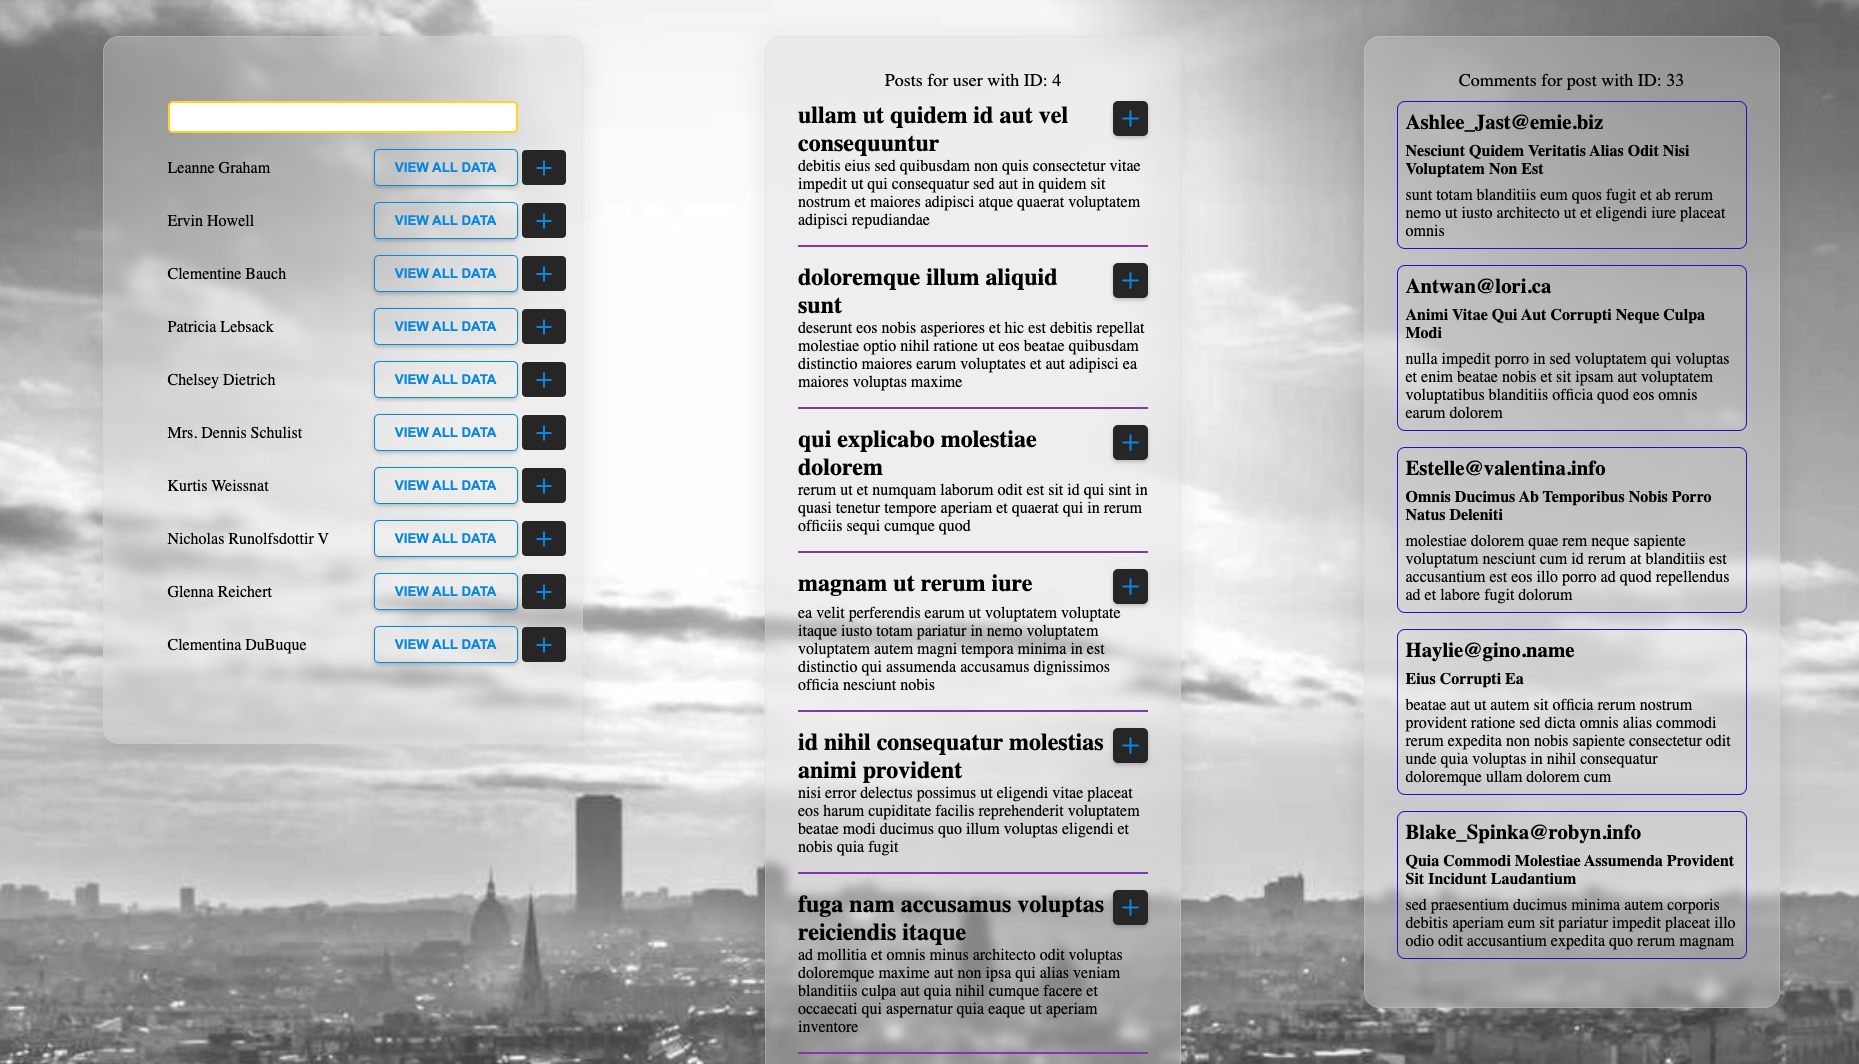
\includegraphics[width=0.9\textwidth]{01_desktop_preview.png}
	\caption{Aplica\c tia practic\u a - vanilla JavaScript}
	\label{fig:preview-vanillajs}
\end{figure}

Pentru a ob\c tine datele de la API, am utilizat func\c tia  \emph{fetch}:
\begin{lstlisting}
	const usersRes = await fetch("https://jsonplaceholder.typicode.com/users");
	const postsRes = await fetch("https://jsonplaceholder.typicode.com/posts");
\end{lstlisting}

Pentru a implementa func\c tionalitatea de afi\c sare a post\u arilor asociate unui utilizator, am utilizat localstorage pentru a stoca Id-ul \c si numele utilizatorului curent, pentru a folosi aceste date \^in func\c tia de filtrare a post\u arilor:
\begin{lstlisting}
	function handleSaveButtonClick(event) {
		localStorage.setItem("selectedUser", JSON.stringify(selectedUser));
	}

	async function renderPosts(data) {
		const postsUl = document.getElementById("posts");
		const selectedName = localStorage.getItem("selectedName");
  		const selectedUser = ALL_USERS.find((user) => user.name === selectedName);

		const html = data.map( (posts) => 
			`<li class="list-item-post"> 
			<h2 class='post-header'> ${post.title} </h2>
			<p> ${post.body} </p>
			</li>`).join("");

	  	postsUl.innerHTML += html;
	}

\end{lstlisting}
\subsection{React}

Cu ajutorul comenzii \emph{npx create-react-app 02-react} se genereaz\u a un proiect React, cu numele 02-react, care va con\c tine fi\c sierele configurate \c si folderele necesare pentru aplica\c tia React, inclusiv structura de baz\u a a proiectului, fi\c sierele de configurare implicite \c si dependen\c tele ini\c tiale.

\begin{figure}[htbp]
	\centering
	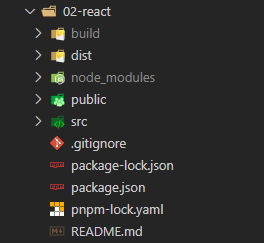
\includegraphics[width=0.4\textwidth]{react_file_structure.png}
	\caption{Structura unei aplica\c tii React}
	\label{fig:react-structure}
\end{figure}

Directorul "src" dintr-un proiect con\c tine fi\c sierele de cod surs\u a pentru aplica\c tia React. Aici sunt scrise \c si organizate componentele, stilurile \c si alte fi\c siere relevante ale aplica\c tiei.

Aplica\c tia construit\u a cu React are c\^ateva avantaje fa\c t\u a de o aplica\c tie construit\u a cu vanilla JavaScript:

\begin{enumerate}
	\item \textbf{Eficien\c t\u a \c si performan\c t\u a}: Virtual DOM permite re-randarea selectiv\u a a componentelor. Virtual DOM-ul este o copie a DOM-ului real, stocat\u a \^in memorie. Atunci c\^and apar modific\u ari \^in starea sau propriet\u a\c tile unei componente, React declan\c seaz\u a un proces de re-randare - se compara Virtual DOM-ul anterior cu cel nou generat pentru componenta afectate \c si descenden\c tii acesteia, folosind procesul de reconciliere. Prin calcularea diferen\c telor (diffing) \^intre cele dou\u a Virtual DOM-uri, React identific\u a p\u ar\c tile specifice care necesit\u a actualizare, apoi aplic\u a doar actualiz\u arile necesare componentelor afectate \^in DOM-ul real, minimiz\^and rand\u arile excesive ale componentelor nemodificate. Capacitatea Virtual DOM-ului de a efectua actualiz\u ari selective contribuie la viteza \c si eficien\c ta React, \^in special \^in gestionarea structurilor complexe de interfa\c t\u a de utilizator \c si a modific\u arilor frecvente ale st\u arii sau propriet\u a\c tilor.
	\begin{figure}[htbp]
		\centering
		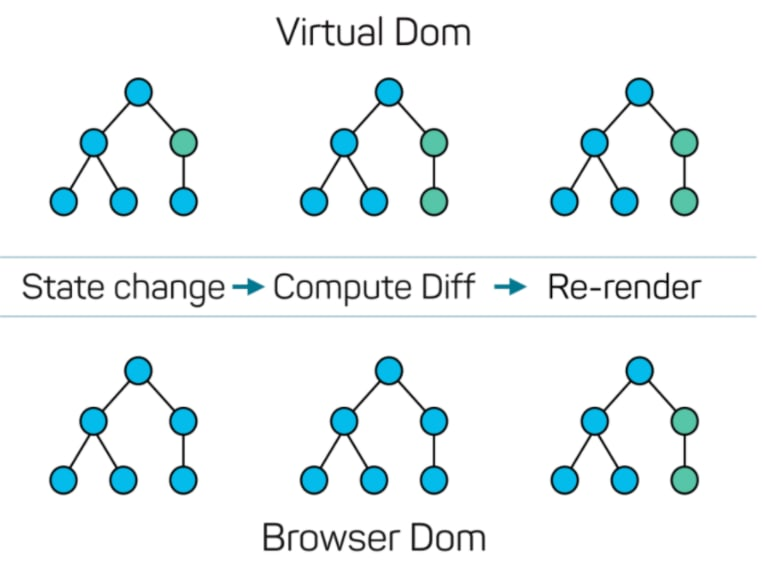
\includegraphics[width=0.6\textwidth]{virtual-dom.jpeg}
		\caption{Ilustrarea procesului de reconciliere}\protect\footnotemark
		\label{fig:virtual-dom}
	\end{figure}

	\footnotetext{ \url{https://dev.to/adityasharan01/react-virtual-dom-explained-in-simple-english-10j6}}
	\item \textbf{Sintax\u a declarativ\u a}: React urmeaz\u a o paradigma de programare declarativ\u a, ce permite dezvoltatorilor s\u a descrie cum ar trebui s\u a arate interfa\c ta utilizator pe baza st\u arii curente a componentelor, \^in loc s\u a manipuleze manual DOM-ul. Aceasta simplific\u a dezvoltarea, \^imbun\u at\u a\c te\c ste lizibilitatea codului \c si reduce probabilitatea apari\c tiei erorilor.
	\item \textbf{React hooks}: ofer\u a o modalitate mai concis\u a \c si intuitiv\u a de a gestiona starea \c si efectele secundare. Cu ajutorul hooks-urilor, componentele func\c tionale pot avea starea local\u a (\textit{hook-ul useState}), pot efectua efecte secundare(\textit{hook-ul useEffect}), pot accesa valorile contextului (\textit{hook-ul useContext}), pot crea referin\c te mutable folosind hook-ul useRef, pot memoiza calculele folosind hook-ul useMemo \c si pot memoiza func\c tiile de callback folosind hook-ul useCallback. Hooks-urile promoveaz\u a reutilizabilitatea codului, \^imbun\u at\u a\c tesc lizibilitatea \c si experien\c ta de dezvoltare, permi\c t\^and dezvoltatorilor s\u a scrie componente mai modulare \c si func\c tionale f\u ar\u a a fi nevoie de componente de tip clas\u a. Acestea au devenit o parte esen\c tial\u a a React-ului, facilit\^and gestionarea logicii \c si a efectelor secundare \^in cadrul componentelor func\c tionale. \cite{react-hooks}
\end{enumerate}

Pentru a re\c tine anumite date, precum utilizatorul curent, masivul de post\u ari sau valoarea curent\u a a input-ului putem utiliza hook-ul \emph{useState}, ce permite gestionarea \c si actualizarea st\u arii interne a unei componente, iar pentru a ob\c tine listele de utilizatori \c si postr\u ari \^intr-un mod efectiv, utiliz\u am hook-ul \emph{useEffect} pentru a ne asigura c\u a acestea sunt executate la momentele potrivite \^in timpul ciclului de via\c t\u a al componentei.

\begin{lstlisting}
	useEffect(() => {
    async function fetchData() {
    	const usersRes = await fetch("https://jsonplaceholder.typicode.com/users");
    	const postsRes = await fetch("https://jsonplaceholder.typicode.com/posts");
      
		const usersData = await usersRes.json();
    	const postsData = await postsRes.json();

    	allUsers.current = usersData;
    	allPosts.current = postsData;
    	setUsers(usersData);
    	setPosts(postsData);
    }
    fetchData();
  }, []);
\end{lstlisting}
\newpage
\subsection{Next.js}
Este un framework pentru backend, bazat pe React. Tot ce se poate realiza \^in React se poate realiza \c si \^in Next.js, \^ins\u a acesta vine cu o serie de caracteristici suplimentare, precum rutarea, apeluri API, autentificare, pre-rendering, SEO, etc. Aceste func\c tionalit\u a\c ti nu sunt disponibile \^in React \^in mod implicit \c si trebuie instalate biblioteci \c si dependin\c te externe, precum React Router pentru a ob\c tine func\c tionait\u a\c ti similare.

Cu ajutorul comenzii \textit{npx create-next-app@latest 03-next} putem crea o aplica\c tie Next.js. Structura ini\c tial\u a a unei aplica\c tii este similar\u a cu cea a unei aplica\c tii React, cu excep\c tia unor fi\c siere suplimentare:
\begin{figure}[htbp]
	\centering
	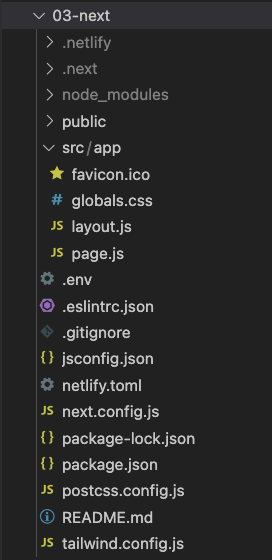
\includegraphics[width=0.45\textwidth]{next_file_structure.png}
	\caption{Structura unei aplica\c tii Next.js}
	\label{fig:next-structure}
\end{figure}


\subsection{Gatsby}
De asemenea este bazat pe React, dar spre deosebire de Next.js este un framework pentru frontend. Gatsby este un generator de site-uri statice, ce permite dezvoltatorilor s\u a creeze site-uri web performante, ce pot fi scalate \c si cu optimizate pentru motoarele de c\u autare. \^In ceea ce prive\c ste capacitatea de gestionare a datelor, Gatsby impune un mod exact \^in care datele trebuie preluate \c si gestionate, cu ajutorul la GraphQL, \^in timp ce Next.js este mai flexibil din acest punct de vedere.

Pentru a crea o aplica\c tie Gatsby, este nevoie de comanda \textit{npm init gatsby}. Structura ini\c tial\u a a unei aplica\c tii:

\begin{figure}[htbp]
	\centering
	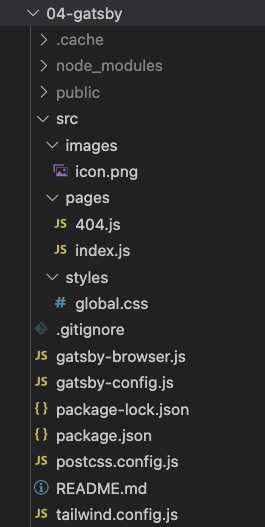
\includegraphics[width=0.47\textwidth]{gatsby_file_structure.png}
	\caption{Structura unei aplica\c tii Gatsby}
	\label{fig:gatsby-structure}
\end{figure}

Folderul \textit{src} este compus din \textit{images}, unde sunt stocate imaginile utilizate, \textit{pages}, unde sunt definite paginile aplica\c tiei \c si folderul \textit{styles}, unde se afl\u a fi\c sierele de stil. Denumirea unui fi\c sier din folderul \textit{pages} reprezint\u a ruta paginii respective. De exemplu, fi\c sierul \textit{index.js} reprezint\u a ruta \textit{/}, iar fi\c sierul \textit{about.js} reprezint\u a ruta \textit{/about}.

Gatsby optimizeaz\u a aplica\c tiile prin utilizarea de plugin-uri, care sunt pachete sau module ce extind func\c tionalitatea Gatsby \c si ofer\u a optimiz\u ari suplimentare. Aceste plugin-uri pot fi folosite pentru \^imbun\u at\u a\c tirea diverselor aspecte ale aplica\c tiei, inclusiv performan\c ta, optimizarea imaginilor \ref{fig:image-optimization}, \^imp\u ar\c tirea codului (\textit{code splitting}), optimizarea SEO.

\section{Analiza performan\c tei}

Performan\c ta aplica\c tiilor a fost testat\u a cu ajutorul Web Vitals, Lighthouse, PageSpeed Insights, dup\u a ce aplica\c tiile au fost \^inc\u arcate pe un web hosting, pentru a ob\c tine o imagine complet\u a \c si obiectiv\u a asupra performan\c tei acestora. 
Rezultatele ob\c tinute ofer\u a informa\c tii detaliate despre performan\c ta aplica\c tiilor, inclusiv timpul de \^inc\u arcare a paginii, interactivitatea, stabilitatea vizual\u a, metode de \^imbun\u at\u a\c tire a acestora \c si o compara\c tie subiectiv\u a a procesului de configurare pentru deploy-ul aplica\c tiilor pe hosting. 

\subsection{Web Vitals}

Toate aplica\c tiile au fost testate dup\u a ce au fost configurate pe acela\c si web hosting - Netlify, \^in condi\c tii de conexiune stabil\u a la internet \c si cu simularea unei conexiuni lente (slow 3G). 

Rezultatele medii ob\c tinute sunt prezentate \^in tabelul urm\u ator:


\begin{table}[htbp]
	\centering
	\begin{tabular}{lcccccccc}
		\toprule
		\multirow{2}{*}{\textbf{Aplica\c tie}} & \multicolumn{4}{c}{\textbf{Conexiune normal\u a}} & \multicolumn{4}{c}{\textbf{3G lent}} \\
		\cmidrule(lr){2-5} \cmidrule(l){6-9}
		& \textbf{LCP} & \textbf{CLS} & \textbf{FID} & \textbf{INP} & \textbf{LCP} & \textbf{CLS} & \textbf{FID} & \textbf{INP} \\
		\midrule
		JavaScript & 0.241s & 0.006 & 0.500ms & 32.000ms & 7.286s & 0.006 & 0.800ms & 16.000ms \\
		React & 0.787s & 0.002 & 0.900ms & 32.000ms & 8.394s & 0.002 & 1.000ms & 16.000ms \\
		Next & 0.448s & 0.002 & 1.100ms & 32.000ms & 10.849s & 0.002 & 1.300ms & 40.000ms \\
		Gatsby & 0.084s & 0.002 & 0.900ms & 16.000ms & 2.127s & 0.002 & 0.900ms & 40.000ms \\
		\bottomrule
	\end{tabular}
	\caption{Rezultatele generate de Web Vitals}
	\label{tab:metrics-web-vitals}
\end{table}

Conform rezultatelor ob\c tinute, aplica\c tia construit\u a cu Gatsby este cea mai eficient\u a din punct de vedere al rand\u arii, urmat\u a de aplica\c tia vanilla JavaScript. Aplica\c tiile construite cu React \c si Next.js au rezultate similare, dar performan\c tele acestora sunt mai slabe. Datorit\u a optimiz\u arilor aduse, \^in special prin utilizarea Gatsby \textit{StaticImage} \c si a \textit{prefetch}-ului, aplica\c tia Gatsby este cea mai rapid\u a din punct de vedere al timpului de randare, at\^at pe conexiunea normal\u a, c\^at \c si pe cea lent\u a.

\subsection{Lighthouse}

Cu ajutorul acestui tool, care este prezent \^in browserele Google Chrome \c si Mozilla Firefox, au fost generate rapoartele de performan\c t\u a pentru aplica\c tiile dezvoltate. Un raport Lighthouse este compus din mai multe sec\c tiuni, fiecare dintre acestea av\^and un scor \c si o descriere a metricilor evaluate. Scorul este calculat pe baza unor ponderi, care sunt diferite pentru fiecare sec\c tiune. Ponderile sunt calculate pe baza unor studii de utilizare, care au fost efectuate de Google.

\begin{figure}[htbp]
	\centering
	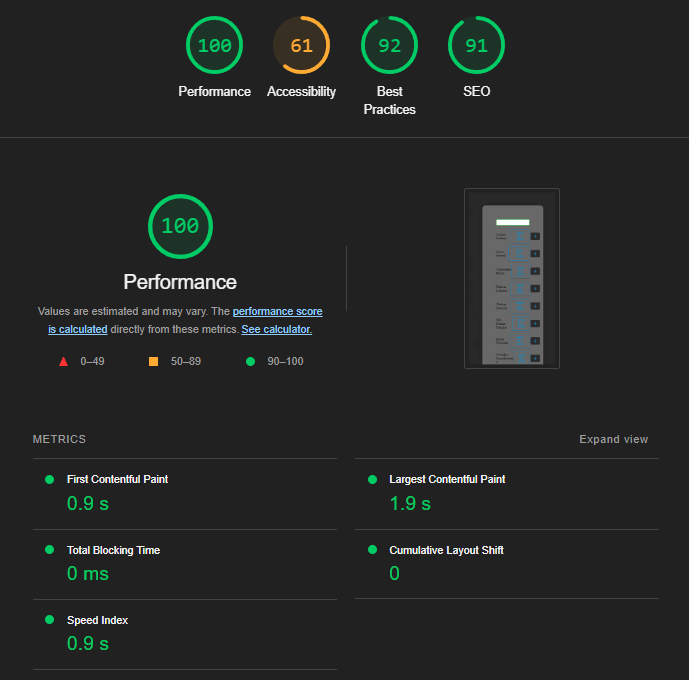
\includegraphics[width=0.75\textwidth]{01_mobile_lighthouse.png}
	\caption{Exemplu raport generat Lighthouse}
	\label{fig:lighthouse-example}
\end{figure}

Pentru fiecare dintre aplica\c tiile dezvoltate au fost generate rapoarte Lighthouse, din case s-au extras cele mai importante metrici, relevante pentru performan\c ta aplica\c tiei \textit{(\textbf{FCP} - First Contentful Paint, \textbf{LCP} - Largest Contentful Paint, \textbf{TBT} - Total Blocking Time, \textbf{CLS} - Cumulative Layout Shift, \textbf{SI} - Speed Index)}, experien\c tei utilizatorului (\textbf{Accessibillity, Best practices}) \c si optimizarea pentru motoarele de c\u autare (\textbf{SEO}). Rezultatele sunt prezentate \^in tabelul urm\u ator:

\begin{table}[htbp]
	\centering
	\begin{tabular}{lccccccccc}
		\toprule
		\multirow{2}{*}{\textbf{Aplica\c tie}} & \multicolumn{4}{c}{\textbf{Performan\c t\u a}} & \multicolumn{4}{c}{\textbf{Alte metrici}} \\
		\cmidrule(lr){2-6} \cmidrule(l){7-9}
		& \textbf{FCP} & \textbf{LCP} & \textbf{TBT} & \textbf{CLS} & \textbf{SI} & \textbf{Accessib.} & \textbf{Best Practices} & \textbf{SEO}\\
		\midrule
		JavaScript & 0.3s & 0.6s & 0 & 0 & 0.9s & 65 & 100 & 89 \\
		React & 0.4s & 0.5s & 0 & 0 & 0.8s & 83 & 100 & 100 \\
		Next & 0.3s & 0.4s & 0 & 0 & 0.4s & 92 & 92 & 100 \\
		Gatsby & 0.2s & 0.2s & 0 & 0 & 0.3s & 82 & 92 & 80 \\
		\bottomrule
	\end{tabular}
	\caption{Rezultatele rapoartelor Lighthouse}
	\label{tab:metrics-lighthouse}
\end{table}

Conform rezultatelor ob\c tinute \^in urma test\u arii, aplica\c tiile dezvoltate cu Next.js \c si Gatsby.js au ob\c tinut cele mai bune rezultate. Aceste scoruri sunt influen\c tate at\^at de optimiz\u arile prezente \^in aceste framework-uri, c\^at \c si de hosting-ul ales, care ofer\u a un mediu de rulare optimizat pentru aplica\c tiile dezvoltate cu Next.js \c si Gatsby. 

Pe baza metricilor analizate, aplica\c tia "Gatsby" demonstreaz\u a o performan\c t\u a mai bun\u a \^in compara\c tie cu celelalte aplica\c tii. Aceasta ob\c tine constant valori mai mici pentru FCP \c si LCP, ce rezult\u a \^intr-o randare mai rapid\u a a con\c tinutului. 

\subsection{PageSpeed Insights}

Evalueaz\u a pagina at\^at pe dispozitive mobile, c\^at \c si pe desktop, atribuie un scor \^in func\c tie de performan\c ta paginii \c si se ofer\u a recomand\u ari pentru \^imbun\u at\u a\c tire. Acest tool ia \^in considerare mai mul\c ti factori care pot afecta performan\c ta unei pagini, cum ar fi timpul de r\u aspuns al serverului, cache-ul resurselor, optimizarea imaginilor, minificarea JavaScript \c si CSS. De asemenea, acesta ia \^in considerare utilizarea celor mai bune practici \c si a ghidurilor de performan\c t\u a web, cum ar fi reducerea resurselor care blocheaz\u a randarea, optimizarea c\u aii critice de randare \c si folosirea cache-ului browserului.

\^In urma test\u arii aplica\c tiilor dezvoltate, au fost ob\c tinute urm\u atoarele rezultate:

\begin{table}[htbp]
	\centering
	\begin{tabular}{lccccccccc}
		\toprule
		\multirow{2}{*}{\textbf{Desktop}} & \multicolumn{4}{c}{\textbf{Performan\c t\u a}} & \multicolumn{4}{c}{\textbf{Alte metrici}} \\
		\cmidrule(lr){2-6} \cmidrule(l){7-9}
		& \textbf{FCP} & \textbf{LCP} & \textbf{TBT} & \textbf{CLS} & \textbf{SI} & \textbf{Accessib.} & \textbf{Best Practices} & \textbf{SEO}\\
		\midrule
		JavaScript & 0.3s & 0.6s & 0 & 0 & 0.9s & 65 & 100 & 89 \\
		React & 0.2s & 0.3s & 0 & 0 & 1.1s & 83 & 100 & 100 \\
		Next & 0.2s & 0.3s & 0 & 0 & 0.7s & 92 & 92 & 100 \\
		Gatsby & 0.2s & 0.2s & 0 & 0 & 0.6s & 85 & 92 & 80 \\
		\bottomrule
	\end{tabular}
	\caption{Rezultatele raport PageSpeed Insights - Desktop}
	\label{tab:metrics-pagespeed-desktop}
\end{table}


\begin{table}[htbp]
	\centering
	\begin{tabular}{lccccccccc}
		\toprule
		\multirow{2}{*}{\textbf{Mobile}} & \multicolumn{4}{c}{\textbf{Performan\c t\u a}} & \multicolumn{4}{c}{\textbf{Alte metrici}} \\
		\cmidrule(lr){2-6} \cmidrule(l){7-9}
		& \textbf{FCP} & \textbf{LCP} & \textbf{TBT} & \textbf{CLS} & \textbf{SI} & \textbf{Accessib.} & \textbf{Best Practices} & \textbf{SEO}\\
		\midrule
		JavaScript & 0.8s & 2.0s & 80ms & 0.102 & 2.2s & 65 & 100 & 91 \\
		React & 0.9s & 1.3s & 250ms & 0 & 2.3s & 83 & 100 & 100 \\
		Next & 0.9s & 0.9s & 190ms & 0 & 1.5s & 92 & 92 & 100 \\
		Gatsby & 0.8s & 0.8s & 50ms & 0 & 1.7s & 85 & 92 & 83 \\
		\bottomrule
	\end{tabular}
	\caption{Rezultatele raport PageSpeed Insights - Mobile}
	\label{tab:metrics-pagespeed-mobile}
\end{table}


\section {Analiza rezultatelor}

Dup\u a ce toate aplica\c tiile au fost construite, acestea au fost \^inc\u arcate pe Netlify - hosting web, ce permite deploy-ul aplica\c tiilor web, scrise \^in diverse limbaje de programare, inclusiv JavaScript \c si framework-uri precum React, Next \c si Gatsby. Pentru ca aplica\c tiile sa ruleze, acestea trebuie configurate, iar complexitatea acestui proces difer\u a de la o aplica\c tie la alta:
\begin{itemize}
	\item \textbf{Vanilla JavaScript} - nu necesit\u a configurare suplimentar\u a, deoarece este un limbaj de programare interpretat, ce ruleaz\u a direct \^in browser. Se poate \^inc\u arca direct folderul ce con\c tine aplica\c tia, iar Netlify va detecta automat fi\c sierele ce trebuie servite \c si va crea un URL public, ce poate fi accesat.
	\item \textbf{React} - este nevoie de pa\c si suplimentari, deoarece este un framework ce necesit\u a un build, pentru a putea fi rulat \^in browser. Pentru a genera build-ul, se folose\c ste comanda "\textit{npm run build}" \^in terminal, ce generEAZ un folder \textit{build}, ce con\c tine toate fi\c sierele necesare rul\u arii aplica\c tiei. Acest folder trebuie \^inc\u arcat pe Netlify.
	\item \textbf{Next.js} - necesit\u a configurare suplimentar\u a, pentru a putea utiliza func\c tionalit\u a\c ti precum server-side rendering sau static site generation. Pentru a genera build-ul, se folose\c ste comanda "\textit{npm run build}" \^in terminal, ce va genera un folder \textit{.next}, ce con\c tine toate fi\c sierele necesare rul\u arii aplica\c tiei. De asemenea este necesar\u a configurarea utiliz\u arii imaginilor preluatre dinamic dintr-un API, prin ad\u augarea unui fi\c sier \textit{next.config.js}:
	\begin{lstlisting}[caption={Configurarea Next.js pentru utilizarea imaginilor dintr-un API},captionpos=b]
		module.exports = {
			images: {
				domains: ['images.unsplash.com'],
			},
		}
	\end{lstlisting}
	\item \textbf{Gatsby} - necesit\u a etape suplimentare de configurare, precum \c si plugin-uri adi\c tionale, ce automatizeaz\u a \c si u\c sureaz\u a procesul de deploy: "\textit{npm install -g gatsby-cli}" \c si "\textit{npm install -D gatsby-plugin-netlify}". De asemenea, este necesar\u a configurarea imaginilor, prin ad\u augarea unui plugin \textit{gatsby-plugin-image} \c si a unui fi\c sier \textit{gatsby-config.js}:
	\begin{lstlisting}[caption={Configurarea Gatsby pentru utilizarea imaginilor dintr-un API},captionpos=b]
		module.exports = {
			plugins: [
				'gatsby-plugin-image',
				'gatsby-plugin-netlify',
				{
				  resolve: 'gatsby-source-filesystem',
				  options: {
					name: 'images',
					path: './src/images/',
				  },
				  __key: 'images',
				},
			  ],
		}
	\end{lstlisting}
\end{itemize}

\subsection{U\c surin\c ta implement\u arii}
Din punct de vedere al utiliz\u arii, vanilla JS este cel mai proeminent, deoarece nu necesit\u a dependen\c te sau framework-uri suplimentare. Pentru a executa un cod JavaScript este destul\u a ad\u augarea unui tag \textit{\textless script\textgreater }   \^ in pagina HTML:
\begin{lstlisting}[caption={Exemplu de ad\u augare a unui script \^ in pagina HTML},captionpos=b]
	<script>
		const exemplu = "Hello World!";
	</script>
	\end{lstlisting}

sau adaugarea unui fi\c sier JavaScript separat, care poate fi inclus \^ in pagina HTML cu ajutorul aceluia\c si tag, dar cu specificarea loca\c tiei fi\c sierului:

\begin{lstlisting}[caption={Exemplu de ad\u augare a unui script dintr-un fi\c sier extern},captionpos=b]
	<script src="path/to/file.js"></script>
\end{lstlisting}

Aplica\c tiile create cu ajutorul framework-urilor React, necesit\u a pa\c si suplimentari pentru configurarea ini\c tial\u a a proiectului folosind \textit{create-react-app} sau configurarea manual\u a a unui mediu de dezvoltare. De asemenea, este necesar\u a instalarea dependen\c telor proiectului, care pot fi gestionate cu ajutorul unui package manager, cum ar fi \textit{npm} sau \textit{yarn}. React utilizeaz\u a JSX - o sintax\u a care combin\u a JavaScript cu HTML, care necesit\u a un preprocesor pentru a fi transformat \^in JavaScript valid.

\begin{lstlisting} [caption={Comparare sintax\u a JSX \c si JavaScript},captionpos=b]
	--- cod JSX
	const numbers = [1, 2, 3, 4, 5];
	const list = (
		<ul>
			{numbers.map((number) => (
			<li key={number}>{number}</li>
			))}
		</ul>
	);
	--- cod JavaScript
	const numbers = [1, 2, 3, 4, 5];
	const list = React.createElement("ul",null,
		numbers.map((number) =>
			React.createElement("li", { key: number }, number)
		)
	);

\end{lstlisting}

JSX \^imbun\u at\u a\c te\c ste lizibilitatea codului prin utilizarea de cod similar HTML \^in cadrul JavaScript. Reprezentarea vizual\u a a structurii codului spore\c ste u\c surin\c ta de \^intre\c tinere \c si debugging-ul.

Promoveaz\u a o abordare modular\u a \c si bazat\u a pe componente, care poate fi reutilizate, facilit\^and crearea \c si gestionarea elementelor de interfa\c t\u a. Componentele pot fi scrise direct \^in cadrul codului JavaScript, permi\c t\^and o organizare eficient\u a a codului \c si reutilizabilitate.

\begin{lstlisting}[caption={Exemplu de component\u a React},captionpos=b]
	function Welcome(props) {
		return <h1>Hello, {props.name}</h1>;
	}
\end{lstlisting}

Next.js \c si Gatsby sunt framework-uri care se bazeaz\u a pe React, oferind un mediu de dezvoltare mai u\c sor, cu un set de func\c tionalit\u a\c ti predefinite, cum ar fi server-side rendering, generarea de pagini statice, optimizarea imaginilor:

\begin{lstlisting}[caption={Exemplu de utilizare a unei imagini optimizate automat \^in Next.js \c si Gatsby},captionpos=b]
	--- Next.js
	import Image from 'next/image'
	function HomeImage() {
		return (
				<Image
					src="https://picsum.photos/1920/1080?grayscale"
					alt="Background picture"
				/>
		)
	}
	export default HomeImage

	
	--- Gatsby
	import React from "react"
	import { StaticImage } from "gatsby-plugin-image"
	const HomeImage = () => {
		return (
				<StaticImage
					alt="Background picture"
					src="https://picsum.photos/1920/1080?grayscale"
				/>
		)
	}
\end{lstlisting} \label{fig:image-optimization}

Acestea sunt utile pentru crearea de aplica\c tii web complexe, care necesit\u a o structur\u a bine definit\u a \c si o arhitectur\u a scalabil\u a, \^ins\u a necesit\u a o perioad\u a de timp mai mare pentru a fi \^inv\u a\c tate \c si implementate.

\subsection{Performan\c ta}

\^In urma analizei rezultatelor ob\c tinute cu ajutorul Web Vitals, rapoartelor generate de Lighthouse \c si PageSpeed Insights se poate observa faptul c\u a aplica\c tia construit\u a cu Gatsby este cea mai performant\u a, datorit\u a optimiz\u arii automate a imaginilor \c si a gener\u arii de pagini statice. \^In cazul aplica\c tiei construite cu Next.js, performan\c ta este influen\c tat\u a de modul de implementare, deoarece nu exist\u a o optimizare automat\u a a imaginilor, iar paginile sunt generate dinamic. Aplica\c tia construit\u a cu vanilla JS este cea mai pu\c tin performant\u a, deoarece nu exist\u a o optimizare a imaginilor, iar codul este scris \^intr-un singur fi\c sier, ceea ce duce la un timp de \^inc\u arcare mai mare.

Pe desktop, Gatsby a reu\c sit s\u a ofere o performan\c t\u a deosebit\u a, cu valori mici pentru FCP (0.2s), LCP (0.2s) \c si o lips\u a total\u a a timpului de blocare semnificativ (TBT = 0). Aceste rezultate indic\u a o experien\c t\u a rapid\u a \c si fluid\u a pentru utilizatorii care acceseaz\u a aplica\c tia Gatsby pe desktop.

\^In ceea ce prive\c ste dispozitivele mobile, Gatsby continu\u a s\u a ofere o performan\c t\u a excelent\u a, ob\c tin\^and valori competitive pentru FCP (0.8s) \c si LCP (0.8s). De\c si valorile sunt u\c sor mai ridicate dec\^at \^in cazul desktopului, Gatsby \^inc\u a se men\c tine \^in fruntea clasamentului, asigur\^and o \^inc\u arcare rapid\u a \c si o experien\c t\u a pl\u acut\u a pe dispozitivele mobile.

\subsection{Dimensiunea aplica\c tiei}

Dimensiunea aplica\c tiei este un alt factor important care influen\c teaz\u a performan\c ta. Cu c\^ at mai mare este dimensiunea aplica\c tiei, cu at\^ at mai multe resurse trebuie desc\u arcate de c\u atre browser, ceea ce duce la un timp de \^ inc\u arcare mai mare. Dimensiunea aplica\c tiei este influen\c tat\u a de framework-ul folosit, bibliotecile suplimentare, dependen\c tele aplica\c tiei \c si de modul de implementare.
\^In urma analizei fi\c sierelor desc\u arcate de c\u atre browser, \^in tab-ul de Network din DevTools, am ob\c tinut urm\u atoarele rezultate:

\begin{itemize}
	\item Vanilla JavaScript \(\sim \) 198.1 KB
	\item React \(\sim \) 255.5 KB
	\item Next.js \(\sim \) 202.2 KB (\textit{f\u ar\u a optimizarea imaginilor}) \c si 138.9 KB (\textit{cu optimizarea imaginilor})
	\item Gatsby \(\sim \) 205.3 KB (\textit{f\u ar\u a optimizarea imaginilor}) \c si 124.7 KB (\textit{cu optimizarea imaginilor}) 
\end{itemize}

Framework-urile Next.js \c si Gatsby au adus o \^imbun\u at\u a\c tire semnificativ\u a \^in ceea ce prive\c ste optimizarea imaginilor, ceea ce a dus la o dimensiune mai mic\u a a aplica\c tiilor \^in compara\c tie cu utilizarea doar a Vanilla JS \c si React. De\c si framework-urile includ mai multe libr\u arii suplimentare, care pot cre\c ste dimensiunea general\u a a aplica\c tiei, func\c tionalit\u a\c tile pe care le ofer\u a acestea sunt optimizate pentru a reduce dimensiunea final\u a a aplica\c tiei.

\subsection{SEO}

Vanilla JS nu ofer\u a suport direct pentru optimizarea pentru motoarele de c\u autare. Implementarea SEO trebuie f\u acut\u a manual, inclusiv gestionarea meta tag-urilor, structurarea con\c tinutului \c si gestionarea URL-urilor.

React ofer\u a suport pentru optimizarea pentru motoarele de c\u autare, prin intermediul unor biblioteci dedicate \c si necesit\u a aten\c tie suplimentar\u a \c si cuno\c stin\c te SEO pentru a implementa aceste optimiz\u ari. Prin utilizarea React Helmet sau a altor biblioteci similare, este posibi\u a ad\u augarea meta tag-urilor relevante.

Next.js are abilit\u a\c ti de optimizare pentru SEO \^incorporate. Ofer\u a suport nativ pentru server-side rendering (SSR) - paginile vor fi preg\u atite \c si livrate c\u atre motoarele de c\u autare cu con\c tinutul complet generat, facilit\^and astfel indexarea \c si clasificarea mai bun\u a \^in rezultatele c\u aut\u arii. Next.js gestioneaz\u a automat meta tag-urile dinamice pentru fiecare pagin\u a \c si, de asemenea, faciliteaz\u a generarea paginilor statice, care pot fi extrem de benefice pentru SEO.

Gatsby este un framework care pune accent pe performan\c t\u a \c si optimizare pentru SEO. Prin generarea paginilor statice \^in avans, Gatsby ofer\u a un avantaj semnificativ \^in ceea ce prive\c ste viteza de \^inc\u arcare a paginilor \c si indexarea lor de c\u atre motoarele de c\u autare. Gatsby are, de asemenea, suport nativ pentru gestionarea meta tag-urilor \c si structurarea con\c tinutului pentru a ob\c tine rezultate optime \^in SEO. De asemenea, Gatsby beneficiaz\u a de integrarea cu GraphQL, permi\c t\^and \^inc\u arcarea eficient\u a a datelor \c si gestionarea optim\u a a con\c tinutului pentru SEO.

\chapter{Concluzii}

Aceast\u a lucrare ofer\u a o perspectiv\u a asupra tehnologiilor de randare \c si a impactului lor asupra aplica\c tiilor web din punct de vedere al performan\c tei, optimiz\u arii \c si experien\c tei utilizatorilor.
Este important de men\c tionat faptul c\u a performan\c ta unei aplica\c tii web nu se rezum\u a doar la tehnologia de randare utilizat\u a, ci \c si la practicile de optimizare \c si \^imbun\u at\u a\c tire continu\u a. Utilizarea instrumentelor precum Lighthouse \c si PageSpeed Insights poate oferi informa\c tii valoroase pentru identificarea punctelor slabe \c si \^imbun\u at\u a\c tirea performan\c tei unei aplica\c tii web.

Alegerea tehnologiei de randare depinde de cerin\c tele specifice ale aplica\c tiei proiectate. SSR \textit{(Server Side Rendering)} ofer\u a avantaje din punct de vedere al SEO, datorit\u a faptului c\u a con\c tinutul HTML este generat direct pe server \c si este furnizat c\u atre motoarele de c\u autare, \^imbun\u at\u a\c tirea performan\c tei \^inc\u arc\u arii ini\c tiale a paginii, dar are dezavantaje \^in ceea ce prive\c ste interactivitatea, deoarece \^intreaga pagin\u a trebuie re\^inc\u arcat\u a pentru a actualiza con\c tinutul. 

CSR \textit{(Client Side Rendering)}, pe de alt\u a parte, ofer\u a o experien\c t\u a mai interactiv\u a, deoarece con\c tinutul este generat \^in browser, dar are dezavantaje \^in ceea ce prive\c ste performan\c ta \^inc\u arc\u arii ini\c tiale a paginii, deoarece \^intregul JavaScript trebuie desc\u arcat \c si executat \^inainte ca pagina s\u a poat\u a fi afi\c sat\u a.

SSG \textit{(Static Server Generation)} este o alternativ\u a la SSR, care ofer\u a avantajele SEO \c si performan\c ta \^inc\u arc\u arii ini\c tiale a paginii, dar nu ofer\u a interactivitatea oferit\u a de CSR. 

\^In ceea ce prive\c ste tehnologiile de randare, React ofer\u a o experien\c t\u a de dezvoltare mai bun\u a, datorit\u a faptului c\u a este mai u\c sor de \^inv\u a\c tat \c si de utilizat, oferind unelte \textit{precum create-react-app}, care ofer\u a un mediu de dezvoltare preconfigurat \c si sintax\u a cunoscut\u a, deoarece este bazat pe JavaScript. Beneficiile care le ofer\u a React sunt cel mai eviden\c tiate \^in aplica\c tiile complexe cu interfe\c te de utilizator dinamice \c si actualiz\u ari frecvente, unde virtual DOM \c si mecanismele eficiente de randare ofer\u a un UX mai bun.

Vanilla JS, pe de alt\u a parte, ofer\u a o performan\c t\u a mai bun\u a, deoarece nu necesit\u a biblioteci suplimentare, dar are o curba de \^inv\u a\c tare mai mare \c si necesit\u a mai mult cod pentru a realiza acelea\c si func\c tionalit\u a\c ti.

Cu toate acestea, este important de men\c tionat c\u a \^in aplica\c tiile mai simple sau \^in cazurile \^in care interactivitatea nu este un aspect major, JavaScript simplu poate fi mai performant datorit\u a naturii sale. Vanilla JavaScript evit\u a costurile suplimentare ale unui framework precum React \c si poate fi optimizat pentru cazuri de utilizare specifice, rezult\^and \^intr-o  execu\c tie mai rapid\u a.

Fiecare dintre metodele abordate are avantajele \c si dezavantajele sale. Vanilla JS este cel mai simplu de implementat, deoarece nu necesit\u a dependen\c te sau biblioteci suplimentare. React este un framework popular, care ofer\u a o abordare mai structurat\u a a dezvolt\u arii aplica\c tiilor web, dar necesit\u a un timp mai mare de implementare \c si configurare. Next.js \c si Gatsby sunt framework-uri construite pe React, care ofer\u a un set de func\c tionalit\u a\c ti suplimentare, ce pot fi utile \^ in dezvoltarea unei aplica\c tii web, dar necesit\u a cuno\c stin\c te mai avansate de React \c si a specifica\c tiilor interne ale acestor framework-uri.

\section{Rezultatele ob\c tinute}

\^In urma analizei perfoman\c tei aplica\c tiilor construite, aplica\c tia dezvoltat\u a cu ajutorul framework-ului Gatsby este cea mai performant\u a, deoarece utilizeaz\u a paradigma SSG (Static Server Generation), care este caracterizat\u a prin generarea con\c tinutului HTML pe server, \^inainte de a fi livrat c\u atre utilizatori. Aceast\u a abordare ofer\u a o performan\c t\u a sporit\u a \^in ceea ce prive\c ste timpul de \^inc\u arcare a paginii, deoarece nu necesit\u a randarea con\c tinutului \^in browser, ci doar livrarea acestuia c\u atre utilizator. De asemenea, datorit\u a optimiz\u arilor oferite de Gatsby, imaginile sunt comprimate \c si redimensionate, iar codul este minificat, ceea ce duce la o performan\c t\u a sporit\u a a aplica\c tiei.

Aplica\c tiile ce au fost construite cu ajutorul React, Next.js \c si Gatsby au o dimensiune mai mare, deoarece necesit\u a biblioteci suplimentare pentru a func\c tiona \c si trebuie configurate pentru a putea fi hostate pe web, fapt ce poate rezulta \^intr-o experien\c t\u a de dezvoltare mai complex\u a, \^ins\u a aceasta este compensat\u a de beneficiile oferite de aceste framework-uri.

\^In aplica\c tia ce utilizeaza vanilla JS, manipul\u arile DOM sunt realizate direct, iar \^in cazul unei aplica\c tii simple aceast\u a abordare direct\u a este mai eficient\u a dec\^at utilizarea React \c si virtual DOM, ce necesit\u a pa\c si suplimentari pentru actualizarea con\c tinutului.

Odat\u a cu scalarea aplica\c tiei, framework-urile devin mai performante, iar codul mai u\c sor de men\c tinut, datorit\u a arhitecturii predefinite, bazate pe componente reutilizabile \c si alte unelte de dezvoltare precum hook-urile, ce simplific\u a implementarea, actualizarea \c si scalarea optim\u a a func\c tionalit\u a\c tilor necesare.

\section {Direc\c tii viitoare de cercetare}

\^In timp ce studiul actual s-a concentrat pe compararea performan\c tei JavaScript-ului simplu (Vanilla), React, Next.js \c si Gatsby \^intr-o aplica\c tie web relativ simpl\u a, exist\u a mai multe direc\c tii pentru cercet\u ari ulterioare, care pot extinde \^in\c telegerea asupra acestor tehnologii de randare \^in scenarii mai complexe. Prin investigarea acestor direc\c tii, putem ob\c tine o perspectiv\u a mai profund\u a asupra punctelor forte \c si limit\u arilor fiec\u arei tehnologii \c si a performan\c tei acestora \^in aplica\c tii web complexe, cu con\c tinut dinamic \c si actualiz\u ari frecvente ale componentelor.

Prin cre\c sterea complexit\u a\c tii \c si a dimensiunii aplica\c tiei, inclusiv ad\u augarea mai multor pagini, va fi posibi\u a evaluarea modului \^in care fiecare tehnologie gestioneaz\u a sarcina de lucru suplimentar\u a. Aceast\u a analiz\u a ar ajuta la determinarea dac\u a anumite tehnologii sunt mai potrivite pentru aplica\c tii de mari dimensiuni \c si ar dezv\u alui eventuale restric\c tii de performan\c t\u a care pot ap\u area.

Acest studiu s-a axat pe utilizarea vanilla JS, React, Next.js \c si Gatsby, \^ins\u a exist\u a numeroase framework-uri \c si tehnologii de randare. Cercet\u arile ulterioare ar putea extinde compara\c tia pentru a include alte framework-uri sau biblioteci, cum ar fi Angular, Vue.js sau Svelte \c si tehnologii de randare precum ISR (\textit{Incremental Static Regeneration}), care este o variant\u a \^imbun\u at\u a\c tit\u a a SSG, \^in care paginile statice se pot regenera pe server la cerere, f\u ar\u a necesitatea de rebuild a \^intregii aplica\c tii. 

Prin includerea unui spectru mai larg de tehnologii de randare, putem ob\c tine o perspectiv\u a mai larg\u a asupra performan\c tei acestora \c si a modului \^in care se compar\u a cu cele evaluate \^in acest studiu.



\renewcommand{\bibname}{Bibliografie}

\bibliographystyle{Plain} % Plain, Abbrv, Unsrt, Alpha
\addcontentsline{toc}{chapter}{Bibliography}

\begin{thebibliography} {21}
	\bibitem{web-1} Mike Evans. \textbf{\textit{“The Evolution of the Web - From Web 1.0 to Web 4.0”}} (2008)
	
	\bibitem{oreilly}Tim O'Reilly. \textbf{\textit{“What Is Web 2.0”}} - \url{https://www.oreilly.com/pub/a/web2/archive/what-is-web-20.html} (2005)
	
	\bibitem{semantic-web}Sean B. Palmer. \textbf{\textit{“The Semantic Web: An Introduction”}} (2001)
	
	\bibitem{pwa}Dennis Sheppard. \textbf{\textit{“Introduction to Progressive Web Apps”}} (2017)

	\bibitem{ajax}Jesse James Garrett. \textbf{\textit{“Ajax: A New Approach to Web Applications”}} (2007)

	\bibitem{virtual-dom}A. Javeed. \textbf{\textit{“Performance Optimization Techniques for ReactJS”}} (2019)

	\bibitem{rendering-patterns}German Cocca. \textbf{\textit{“Rendering Patterns for Web Apps - Server-Side, Client-Side, and SSG Explained”}} - \url{https://www.freecodecamp.org/news/rendering-patterns/} (2023)
	
	\bibitem{choose-rendering}\textbf{\textit{“Choose the Rendering Method (SPA vs SSR vs SSG)”}} - \url{https://dev.to/crunchstack/choose-the-rendering-method-spa-vs-ssr-vs-ssg-121f} (2021)
	
	\bibitem{lcp}Philip Walton, Barry Pollard. \textbf{\textit{“Largest Contentful Paint (LCP)”}} - \url{https://web.dev/lcp/} (2019)
	
	\bibitem{cls}Philip Walton, Milica Mihajlija. \textbf{\textit{“Cumulative Layout Shift (CLS)”}} - \url{https://web.dev/cls/} (2019)
	
	\bibitem{fid}Philip Walton. \textbf{\textit{“First Input Delay (FID)”}} - \url{https://web.dev/fid/} (2019)

	\bibitem{inp}Jeremy Wagner. \textbf{\textit{“Interaction to Next Paint (INP)”}} - \url{https://web.dev/inp/} (2019)

	\bibitem{web-vitals}Barry Pollard, Michal Mocny, Rick Viscomi, Brendan Kenny. \textbf{\textit{“Using the Web Vitals extension to debug Core Web Vitals issues”}} - \url{https://web.dev/debug-cwvs-with-web-vitals-extension/}(2023)
	
	\bibitem{lighthouse}Tushar Pol. \textbf{\textit{“Google Lighthouse: What It Is \& How to Use It”}} - \url{https://www.semrush.com/blog/google-lighthouse/}(2023)
	
	\bibitem{pagespeed-insights}Google documentation. \textbf{\textit{“About PageSpeed Insights”}} - \url{https://developers.google.com/speed/docs/insights/v5/about}
	
	\bibitem{react-hooks}John Larsen. \textbf{\textit{“React Hooks in Action: With Suspense and Concurrent Mode”}}, p.[54,96,121] (2021)

	\bibitem{benefitsserverrendering} Alex Grigoryan. \textbf{\textit{“The Benefits of Server Side Rendering Over Client Side Rendering”}} - \url{https://medium.com/walmartlabs/the-benefits-of-server-side-rendering-over-client-side-rendering-5d07ff2cefe8} (2017)

	\bibitem{html} Tim Berners-Lee, Daniel Connolly. \textbf{\textit{“Hypertext markup language (html)”}} (1993)

	\bibitem{clientsidevssercerside} Sergey Laptick. \textbf{\textit{“Client Side vs Server Side UI Rendering. Advantages and Disadvantages”}} -  \url{https://blog.webix.com/client-side-vs-server-side-ui-rendering/} (2017)

	\bibitem{improve-ssr-speed} Anna Monus. \textbf{\textit{“What Is Server-side Rendering And How Does It Improve Site Speed?”}} -  \url{https://www.debugbear.com/blog/server-side-rendering} (2019)

	\bibitem{google-bouncing-rate} Google Research - \url{https://www.thinkwithgoogle.com/marketing-strategies/app-and-mobile/mobile-page-speed-new-industry-benchmarks-load-time-vs-bounce/} (2017)


\end{thebibliography}


\appendix % begin appendix part

\chapter{Glosar}


\section{Acronime}

\begin{table} [H]
	\begin{tabular} {|  l | L{10cm} |}
		\hline
		SSR & Server side rendering      \\ [0.2ex]
		\hline
		CSR & Client side rendering      \\ [0.2ex]
		\hline
		SSG & Static server generation   \\ [0.2ex]
		\hline
		UX  & User experience            \\ [0.2ex]
		\hline
		UI  & User interface             \\ [0.2ex]
		\hline
		LCP & Largest contentful paint   \\ [0.2ex]
		\hline
		FID & First input delay          \\ [0.2ex]
		\hline
		CLS & Comulative layout shift    \\ [0.2ex]
		\hline
		SEO & Search engine optimization \\ [0.2ex]
		\hline
		JS  & JavaScript                 \\ [0.2ex]
		\hline
	\end{tabular}
	\caption{Tabel\u a de acronime}
	\label{table:acron}
\end{table}

% end appendix part

\end{document}
